\documentclass[UTF8,a4paper,12pt]{ctexart}
\usepackage{indentfirst}
\usepackage{caption}
\usepackage{chngcntr}
\counterwithout{table}{section}
\usepackage{booktabs}
\usepackage{algorithm} %format of the algorithm 
\usepackage{algorithmic} %format of the algorithm 
\usepackage{ctex}
\usepackage{amsmath}
\numberwithin{equation}{section}
\allowdisplaybreaks[4]       %多行公式中换页
\usepackage{array}
\usepackage[font=small,font=bf,labelsep=none]{caption}
\usepackage{amssymb}
\usepackage{tikz}
\usepackage{amsthm}
\usepackage{mathrsfs}
\usepackage{dutchcal}
\usepackage{color}
\usepackage{graphicx}    %插入图片
\usepackage{times}
\usepackage{mathptmx}
\usepackage{fancyhdr} %页眉页脚
\pagestyle{fancy}
\fancyhf{}
\fancyfoot[C]{\thepage}
\usepackage{setspace}
\setlength{\baselineskip}{20pt}
\newcommand*{\circled}[1]{\lower.7ex\hbox{\tikz\draw (0pt, 0pt)%
    circle (.5em) node {\makebox[1em][c]{\small #1}};}}
\usepackage{hyperref}  %目录
\hypersetup{colorlinks=true,linkcolor=black}
\renewcommand {\thefigure} {\thesection{}-\arabic{figure}}%设定图片的编号。这样设置的实现效果为图1-1
\renewcommand {\thetable} {\thesection{}-\arabic{figure}}
\usepackage{caption}
\captionsetup{font={small},labelsep=quad}%文字5号,之间空一个汉字符位。
\captionsetup[table]{font={bf}} %表格表号与表题加粗
\usepackage{appendix}
\usepackage{tocloft} 
\renewcommand{\cftsecleader}{\cftdotfill{\cftdotsep}} %为目录中section补上引导点
\usepackage{titletoc}
\titlecontents{section}[0pt]{\addvspace{6pt}\filright\bf}%
               {\contentspush{\thecontentslabel \quad}}%
               {}{\titlerule*[8pt]{.}\contentspage}
\makeatletter %双线页眉
\def\headrule{{\if@fancyplain\let\headrulewidth\plainheadrulewidth\fi%
\hrule\@height 1.5pt \@width\headwidth\vskip1.5pt%上面线为1pt粗
\hrule\@height 0.5pt\@width\headwidth  %下面0.5pt粗
\vskip-2\headrulewidth\vskip-1pt}      %两条线的距离1pt
  \vspace{6mm}}     %双线与下面正文之间的垂直间距
\makeatother
\CTEXsetup[format={\heiti \zihao{3} \bfseries \center}]{section}
\CTEXsetup[number={第\chinese{section}章}]{section} 
\usepackage[explicit]{titlesec}
\titlespacing*{\section}{0pt}{24pt plus .24pt minus .24pt}{18pt plus .0ex}

\begin{document}

\thispagestyle{empty}

\renewcommand{\headrulewidth}{0pt}
\begin{figure}[htb] 
 \center{
\includegraphics[width=5cm]  {fig1.png}} 
 \end{figure}

\begin{center}
\songti \zihao{-2} 上海交通大学学位论文
\end{center}
%该页为中文扉页。无需页眉页脚,纸质论文应装订在右侧
~\\
\begin{center}
\songti \zihao{1} \textbf{面向有线/无线异构网络的混合时钟同步方法}
\end{center}
%中文论文标题,1行或2行,宋体,加粗,二号,居中。论文题目不得超过36个汉字
~\\
~\\
~\\
~\\
\begin{center}
\heiti \zihao{4}
\begin{tabular}{l}
\textbf{姓\quad名:陈相}\\
\textbf{学\quad号:119032910097}\\
\textbf{导\quad师:陈彩莲}\\
\textbf{学\quad院: 电子信息与电气工程学院}\\
\textbf{学科/专业名称:控制工程}\\
\textbf{申请学位层次:工程硕士}\\
\end{tabular}
\end{center}
\vfill
\vspace{1em}

\begin{center}
\songti \zihao{4} \textbf{2023年5月}
\end{center}

\newpage
\thispagestyle{empty}
~\\
\begin{center}
\zihao{4}
\textbf{
A Dissertation Submitted to \\
Shanghai Jiao Tong University for Master/Doctoral Degree}
\end{center}
~\\
\begin{center}
\zihao{-2}\textbf{
Hybrid Clock Synchronization Method for Wired/Wireless Heterogeneous Networks}
\end{center}
%英文论文标题:大写,Times New Roman,加粗,14 points,居中
~\\
~\\
~\\
\begin{center}
\zihao{3} 
Author:Xiang Chen  \\
Supervisor: Cailian Chen 
\end{center}
~\\
~\\
~\\
\begin{center}
\zihao{3} 
School of Electronic Information and Electrical Engineering \\
Shanghai Jiao Tong University \\
Shanghai, P.R.China \\
May 6th, 2023  
\end{center}

\newpage
\thispagestyle{empty}
\begin{center}
\heiti \zihao{3}\textbf{
上海交通大学\\
学位论文原创性声明}
\end{center}

\zihao{-4}
本人郑重声明:所呈交的学位论文,是本人在导师的指导下,独立进行研究工作所取得的成果。除文中已经注明引用的内容外,本论文不包含任何其他个人或集体已经发表或撰写过的作品成果。对本文的研究做出重要贡献的个人和集体,均已在文中以明确方式标明。本人完全知晓本声明的法律后果由本人承担。

\begin{flushright}
\begin{tabular}{l}
\zihao{4}
学位论文作者签名:\hspace{20mm}\qquad\\
\zihao{4}
日期:\qquad年\qquad月\qquad日
\end{tabular}
\end{flushright}

~\\
\begin{center}
\heiti \zihao{3}\textbf{
上海交通大学\\
学位论文使用授权书}
\end{center}

本人同意学校保留并向国家有关部门或机构送交论文的复印件和电子版,允许论文被查阅和借阅。\\
本学位论文属于 :\par
□公开论文\par
□内部论文,保密□1年/□2年/□3年,过保密期后适用本授权书。\par
□秘密论文,保密\_\_\_年(不超过10年),过保密期后适用本授权书。\par
□机密论文,保密\_\_\_年(不超过20年),过保密期后适用本授权书。\par
(请在以上方框内选择打“√”)\\

\begin{flushright}
\zihao{4}
\begin{tabular}{l l}
学位论文作者签名:\hspace{10mm}\qquad \hspace{100mm}&指导教师签名:\qquad\\
日期:\qquad年\qquad月\qquad日 &日期:\qquad年\qquad月\qquad日\\
\end{tabular}
\end{flushright}

\newpage
\pagenumbering{Roman}
\fancyhead[LH]{上海交通大学学位论文}
\fancyhead[RH]{第一章\quad绪论}

\addcontentsline{toc}{section}{摘\quad要}
\section*{摘\quad要}


近年来,随着工业自动化和物联网的高速发展,分布式系统之间的高精度协同控制需求日益激增,作为协同控制基础的时钟同步也受到了学术界的广泛关注。由于分布式系统复杂的网络环境,存在各种拥塞和排队延迟且节点数量和拓扑结构可能随时发生变化,这使得针对分布式系统的异构网络时钟同步任务充满挑战。因此,本文致力于针对大规模复杂网络,设计出一种以5G-TSN为核心网络的混合架构,并在该架构中实现低复杂度,高精度和抗干扰能力强的跨域时钟同步,以满足大规模复杂异构网络中的适用性、动态性、可扩展性、安全性和鲁棒性等需求。论文的主要工作总结如下:

其一,本文提出了一种针对大规模复杂的有线/无线网络混合时钟同步架构设计:本文首先讨论了时钟模型和时延模型,并引入名为“网络同步性能指标(NSPI)”的综合评估指标,用于网络分层,以便整合异构网络。分层算法将问题建模为有向图,采用预处理方法进行处理,实现井然有序的时钟同步。完成分层后,可以根据最小生成树和分层信息分析网络的同步性能,并在需要时进行优化。混合架构同时也会按照周期进行校验更新,以应对大规模网络中节点参数和网络拓扑变化的问题。实验表明,该混合架构下的时钟同步精度拥有更快的收敛速率与更高的稳定性。

其二,本文针对混合架构核心网络的5G-TSN网络,提出了以新的载波间隔分配优化与时间戳补偿技术。5G+TSN时钟同步在异构网络中具有重要意义,可为各种应用提供高同步精度和低同步延迟。现有的5G与TSN融合同步方案主要关注基站和TSN设备间的协调同步,尚未解决无线网络内部的累积同步误差问题。当前的研究仅考虑单个 5G 网桥的简化情况, 然而,在大规模复杂网络中,多个网桥的应用场景会增加累积同步误差,从而降低时钟同步的准确性。 为了解决这个问题,本文从载波间隔和时间戳两个角度出发进行了同步算法优化,实验表明,该同步方案在保证5G网络带宽利用率的前提下,实现了5G+TSN网络的高精度时间同步。

其三,本文针对5G网络的高速度、大带宽和动态复杂信道环境的特点,设计了自适应判决反馈均衡器(Adaptive Decision Feedback Equalizer, ADFE)。在5G-TSN网络中,为了保持同步精度,通常需要选择较高的载波间隔来实现高精度同步精度,过高的载波间隔会造成多径衰落,从而使得同步稳定性降低。引入ADFE可以有效解决该问题,实验通过比较ADFE与普通均衡器的误码率信噪比曲线,说明了ADFE在5G网络中的5G网络中的优势,包括收敛速度和抗干扰性能。

以上研究表面,基于混合架构的时钟同步拥有较高的同步精度和较强的稳定性,在无线/有线异构网络时钟同步中具有显著的优势,是异构网络时钟同步技术在大规模分布式系统中的一次成功应用。
%摘要:二字间空一格,黑体16磅加粗居中,单倍行距,段前24磅,段后18磅。
\hspace{8mm}\\
~\\
\textbf{关键词}:时钟同步,分布式系统,5G-TSN网桥,混合架构,异构网络\\
%关键字:宋体12磅,行距20磅,段前段后0磅,关键字之间用逗号隔开,关键词三个字加粗。

\newpage
\addcontentsline{toc}{section}{ABSTRACT}
\section*{ABSTRACT}

In recent years, with the rapid development of industrial automation and the Internet of Things, the demand for high-precision cooperative control between distributed systems is increasing, and the clock synchronization as the basis of cooperative control has also received extensive attention from the academic community. Due to the complex network environment of distributed systems, there are various congestion and queuing delays and the number of nodes and topology may change at any time, which makes the task of heterogeneous network clock synchronization for distributed systems is challenging. Therefore, this paper is dedicated to designing a hybrid architecture with 5G-TSN as the core network for large-scale complex networks, and implementing low-complexity, high-precision and interference-resistant cross-domain clock synchronization in this architecture to meet the requirements of applicability, dynamics, scalability, security and robustness in large-scale complex heterogeneous networks. The main work of the paper is summarized as follows:

First, this paper proposes a hybrid clock synchronization architecture design for large-scale complex wired/wireless networks: this paper first discusses the clock model and delay model, and introduces a comprehensive evaluation metric called "Network Synchronization Performance Index (NSPI)" for network layering in order to integrate heterogeneous networks. The layering algorithm models the problem as a directed graph and uses preprocessing methods to achieve well-ordered clock synchronization. Once the layering is completed, the synchronization performance of the network can be analyzed based on minimum spanning tree and layering information and optimized when needed. The hybrid architecture also performs checksum updates according to cycles to cope with node parameters and network topology changes in large-scale networks. Experiments show that the clock synchronization accuracy under the hybrid architecture has a faster convergence rate and higher stability.

Second, this paper proposes a new carrier interval allocation optimization and timestamp compensation technique for 5G-TSN networks with hybrid architecture core networks. 5G+TSN clock synchronization is important in heterogeneous networks to provide high synchronization accuracy and low synchronization delay for various applications. Existing 5G and TSN convergence synchronization schemes focus on the coordinated synchronization between base stations and TSN devices, and have not yet addressed the cumulative synchronization error within the wireless network. The current study only considers the simplified case of a single 5G bridge, however, the application scenario of multiple bridges in a large-scale complex network increases the cumulative synchronization error and thus reduces the accuracy of clock synchronization. To solve this problem, this paper optimizes the synchronization algorithm from two perspectives of carrier interval and timestamp, and experiments show that the synchronization scheme achieves high-precision time synchronization of 5G+TSN networks while ensuring the bandwidth utilization of 5G networks.

Third, this paper designs the Adaptive Decision Feedback Equalizer (ADFE) for the characteristics of high speed, large bandwidth and dynamic and complex channel environment of 5G networks. In 5G-TSN networks, in order to maintain the synchronization accuracy, it is usually necessary to select a high carrier spacing to achieve high precision synchronization accuracy, and too high a carrier spacing will cause multipath fading, thus making the synchronization stability reduced. The introduction of ADFE can effectively solve this problem, and the experiments illustrate the advantages of ADFE in 5G networks including convergence speed and anti-interference performance by comparing the BER signal-to-noise ratio curves of ADFE with those of ordinary equalizers.

The above research surface, based on the hybrid architecture of clock synchronization has a high synchronization accuracy and strong stability, in the wireless / wired heterogeneous network clock synchronization has significant advantages, is a successful application of heterogeneous network clock synchronization technology in large-scale distributed systems.
%ABSTRCT:Arial 16磅加粗居中,单倍行距,段前24磅,段后18磅

\hspace{8mm} \par 
%英文摘要内容:Times New Roman 12磅,行距20磅段前段后0磅
~\\ 
\textbf{Key words}:Clock synchronization, distributed systems, 5G-TSN bridges, hybrid architectures, heterogeneous networks 
%Keywords:Times New Roman 12磅,行距20磅, “key words” 两词加粗

\newpage
\renewcommand\contentsname{\textbf{目\quad录}}
\begin{center}
{\tableofcontents
\thispagestyle{fancy}
\fancyhead [RO, LE] {\normalsize{\songti 第一章\quad绪论}}
\fancyhead [LO, RE] {\normalsize{\songti 上海交通大学学位论文}}
}
\end{center}

\newpage
\pagenumbering{arabic}
\counterwithin{figure}{section}
\counterwithin{table}{section}
\section{绪论}
\subsection{研究背景}
时钟同步是指在分布式系统和网络中,使得各个节点的时钟保持一致的过程。在这个过程中,各个节点通过相互之间的信息交换和调整,使得它们的时钟值尽量接近一个公共的参考时间\textsuperscript{\cite{kopetz1987clock}}。时钟同步是一种关键技术,它确保分布式系统和网络中的各个节点能够协同工作,保持对时间的一致性。在许多应用领域中,例如通信网络、分布式计算和协同控制等,准确的时钟同步对于保障网络数据的有效传输和处理至关重要。从宏观角度来看,时钟同步在网络传输中具有以下重要性:
\begin{itemize}
	\item 数据一致性:在分布式系统中,各个节点之间需要交换数据以完成特定任务。准确的时钟同步确保了节点之间数据的时序一致性,从而避免了因为时间不同步引起的数据错误或丢失。
	\item 事件排序:分布式系统中的事件需要按照正确的顺序进行处理,以确保系统的稳定性和正确性。时钟同步为事件提供了一个全局的时间参考,有助于对事件进行排序和调度。
	\item 协同控制:在一些实时应用场景中,例如无人机编队、智能电网等,多个设备需要协同工作,共同完成任务。时钟同步使得这些设备能够在相同的时间基准下进行协调,从而提高系统的整体性能。
\end{itemize}

近年来,诸如工业自动化,IoT(Internet of Things)之类的技术增长了许多倍,分布式系统的应用变得至关重要\textsuperscript{\cite{7879243}},作为分布式系统协作基础的时钟同步也越来越受到重视。同时,云计算和高速网络的兴起要求高度精确的时间同步\textsuperscript{\cite{CHEN20143}}。廉价的振荡器或石英晶体的特性会随功率,老化和热量的变化而变化。因此,不能保证两个相似的晶体以相同的时间和频率振荡。这些限制使振荡器的运行与其他振荡器略有不同。对于大型基础架构而言,用昂贵的时钟代替计算机的内置廉价时钟是不可行的。因此,一种有力而有效的方式来同步已传播结构的时钟是必不可少的\textsuperscript{\cite{8278257}}。NTP(Network Time Protocol)是时钟同步的最广泛使用的解决方案。后来,一种更精确的解决方案称为PTP(Precise Time Protocol),已被证明对时钟同步更有利\textsuperscript{\cite{5223605}}。尽管PTP通信算法与NTP类似,但PTP在事件的精确硬件辅助时间记录上却有所不同,称为时间戳\textsuperscript{\cite{ahmed2018survey}}。 PTP是可以实现高精度时钟同步的一种可行解决方案。时钟同步是工业网络中非常重要的一环,而且对于时钟同步的要求也是越来越高的,其中无线和有线的时钟同步精度也是有着较大的差别。在有线领域,早期NTP的时钟同步精度由于是协议层的时间戳,误差一般达到$10\mu s$以上,再后来1588的时钟同步利用硬件时间戳,将精度提到到了几十纳秒到几十亚微秒间,同时减少了时钟同步对外部GPS信号的依赖,现在TSN(Time Sensitive Network)的IEEE 802.1AS使用1588的同步方案,同时完全使用mac层进行信息交互,减少了各层级之间的延迟误差,将同步精度稳定在了纳秒级,在具体的工业网络场景中,例如在现有的工业控制网络ethercat中,利用“分布时钟”机制,可以实现小于$1 \mu s$的时钟同步精度\textsuperscript{\cite{idrees2020ieee}}。在无线领域,时钟同步由于无线情况下的能量约束,本身报文时间粒度不高,传输过程中的干扰,本身同步精度要求不高等问题,精度一直停留在微秒级别。但是在5G的应用场景例如载波聚合,多点协同中,同步精度则要求达到100ns级别\textsuperscript{\cite{jakovetic2014fast}}。


TSN由于其高确定性网络而由于成为当前热门,TSN作为时间敏感网络,拥有诸如Qbv等门控调度算法保护来保证时间敏感流的传输,现在做调度算法的有很多,但有一个假设前提:时钟同步是完美的,不存在同步误差和误差抖动;但是,在实际工业场景中假设不成立。TSN对于时钟同步的精度要求极高(ns级别),目前的TSN的同步协议802.1AS,在可接受的误差范围内,有线网络可以提供高精度的时钟同步,但是当网络规模较大,跳数增多,背景流量增多时,同步精度会大幅下降,从而影响整个TSN的性能。\textsuperscript{\cite{ieee2011ieee}}换言之,TSN本身收到有线网络的局限性,需要通过与无线异构来解决有线跳数过多的问题,且在工厂内部的复杂环境下,本身就可能存在的多种无线设备与有线设备异构的情况,仅仅通过保证TSN有线网络内部的高精度同步无法满足实际的应用场景。为将TSN和无线网络相互结合,需要进一步考虑异构网络下的时钟同步方法,可以通过双层网络架构来降低网络规模对于整个同步精度的影响,也就是TSN+无线解决方案,即上层GM(Grand Master)到基站采用有线TSN结构,下层采用无线网络来同步从节点,这种情况下,无线网络的高覆盖性,可以有效降低网络规模较大的情况下跳数对于同步精度的影响,为TSN提供了一个更加有实际意义的应用场景。

而这就涉及到异构网络时钟同步的问题。事实上,异构网络时钟同步随着现在网络规模的增加也在变得越来越重要。有线和无线异构网络中时钟同步的重要性主要体现在以下几个方面:
\begin{itemize}
	\item 系统协调性:在异构网络中,有线和无线节点共同组成一个大的系统。这些节点需要协同完成各种任务,如数据传输、计算和控制等。时钟同步能够确保各个节点在执行任务时具有相同的时间基准,从而提高整个系统的协调性和执行效率。
	\item 数据一致性:在许多应用场景中,如物联网、传感器网络和通信系统等,数据需要在不同的节点之间传递和处理。时钟同步可以保证各个节点在处理数据时具有一致的时间戳,从而确保数据在整个系统中的一致性。
	\item 时延测量与估计:在异构网络中,时延对于性能优化、拥塞控制和质量保证等方面具有重要作用。时钟同步使得各个节点能够准确地测量和估计时延,从而为网络优化提供可靠的依据。
	\item 故障诊断与恢复:时钟同步可以帮助异构网络中的节点快速定位和诊断故障,从而实现快速恢复。这对于保证网络稳定性和可靠性具有重要意义。
\end{itemize}

针对这种有线无线网络异构结构,这些年也有很多时钟同步方案被提出,用来解决异构网络的协同问题,不同的同步方法有着其适用的范围,而对于大规模无线网络节点的异构同步方案,目前没有比较好的同步解决方案。

\subsection{研究现状}
\subsubsection{有线网络的时钟同步问题研究现状}

有线网络部分的时钟同步,目前精度最高的有线网络同步为时间敏感网络的同步方案,时间敏感网络(Time Sensitive Network),简称TSN,采用TSN中协议IEEE 802.1AS规定的时钟同步方案,此此方案是根据IEEE 1588时钟同步方案改进而来,采用主从式同步方法,主从节点之间通过交换时间戳进行上下行延迟进行测量,得到两节点之间的传输延迟,进一步得到时钟偏差。事实上,两节点之间的传输延迟由报文传播延迟,高斯噪声,不确定性延迟组成,后两者是造成时钟同步精度误差的主要原因。在有线网络中,由于较高的稳定性和较好的传输性能,这两部分一般选择忽略不计,即将上下行传输延迟作为对称延迟来进行处理\textsuperscript{\cite{teener2008overview}}。IEEE 802.1AS 协议源自于1588v2时钟同步协议,其原理如下:
\paragraph{1588v2协议}
1588v2是目前最被广泛使用的精密时钟同步协议,全称为IEEE P1588 DM2.2, Standard for a Precision Clock Synchronization Protocol for Networked Measurement and Control Systems,简称为PTP协议,其思路为通过记录时间戳计算网络中的延时误差进行修正,从而达到同步的目的,精度可达ns级。

\begin{figure}[htb] 
	\center{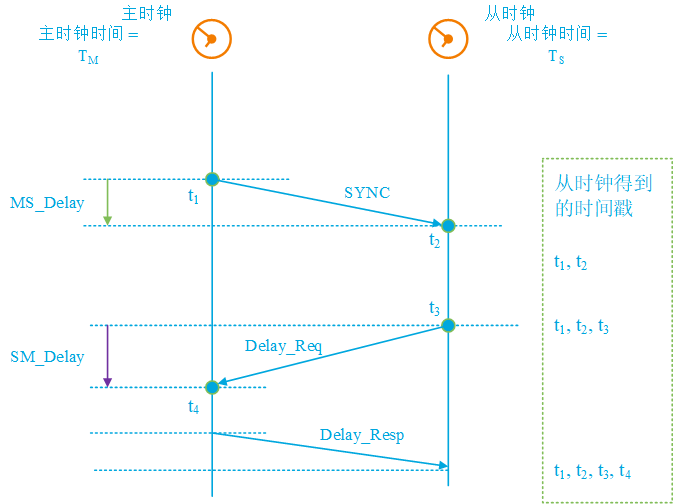
\includegraphics[width=0.95\textwidth]  {fig4.png}} 
	\caption{1588v2同步原理\textsuperscript{\cite{shereen2019next}}}
\end{figure}

延时计算公式为
\begin{equation}
	D = \frac{((t_2-t_1)+(t_4-t_3))}{2} 
\end{equation}
1588v2支持三种时钟类型,普通时钟(Ordinary Clock,OC),边界时钟(Boundary Clock, BC),透明时钟(Transparent Clock,TC),其中5G网桥即利用了透明时钟的概念来实现对驻留时间的修正。
\paragraph{1588v2的局限性}
1588v2可支持高精度的相位同步,可满足5G同步需求。但是在实际应用中,,分组传输网络需要所有节点都支持PTP协议,组网较为复杂,网络的拥塞,时延,抖动,丢包都会影响时钟精度。更为重要的是,1588v2同步需要上下行链路的时延相等,否则就需要人工校准,这一点在项目实施中非常困难,

\subsubsection{无线网络中的时钟同步研究现状}
相比于有线情况的时钟同步,无线网络中的能量约束,以及节点之间的传输干扰,造成无线时钟同步的误差较大。高精度的无线时钟同步的研究目前主要针对WSN和5G。

如果是倾向于高精度的无线时钟同步方案,在同步方法上,更多是采用类似1588的上下报文测量传输延迟的同步方案,在网络结构上,更多是采用类似于聚类的网络结构。聚类网络结构时钟同步的出发角度有从能量的角度出发进行考虑的,也有单纯从精度的角度出发进行考虑的。精度的方面,Xiangli Jia和Yang Lu针对网络跳数对于同步精度的影响做了专门的分析,得出了聚类网络结构相对于传统多跳网络结构的优势\textsuperscript{\cite{jia2019improved}}。Jie Wu,Liyi Zhang则在聚类网络的结构基础上,提出了通过计算共识时钟来进行同步的方案\textsuperscript{\cite{wu2014cluster}}。从能量的角度出发进行考虑的聚类网络结构,更多是从聚类算法的角度进行研究。Pengyi Jia提出通过时钟频率抖动的大小s来进行网络聚类,通过将性能较差的时钟节点聚类进行同步的方式,可以有效降低网络整体的时钟同步频,从而达到降低网络整体能耗的目的\textsuperscript{\cite{jia2019distributed}}。Parminder Kaur也在文章中提出可以通过就近原则的聚类方法,来降低所有节点间通信距离差的和,来达到降低能耗的目的\textsuperscript{\cite{kaur2015energy}}。


针对传统的WSN网络中的聚类时钟同步在现实的应用问题,文献\textsuperscript{\cite{lee2011accuracy}}  等人研究了这些聚类结构时钟同步在5G中的可行性,并提出了可能存在的挑战以及可能的解决方案。5G下的时钟同步,主要是通过BS来完成上层与下层网络之间的同步。但是目前用来传输时间信息的报文SIB16时间精度不高,这就造成了影响时间同步精度关键的时间戳精度不高,而且无线时钟同步方案的时间戳采用的是应用层的时间戳,应用层时间戳在产生过程中很可能会产生较大的非确定性延迟,例如排队延迟,这类延迟通常数量级较大,在传统时钟同步方案中由于产生概率较低,通常放弃对这部分延迟的建模,但是当网络规模增大时,这类延迟的产生概率也会随着增加,从而对时钟同步精度产生较大的影响。如果要实现像TSN的802.1AS一样的高精度时间同步,必须对这一类延迟进行建模补偿,从而才能使得无线网络和有线TSN时钟同步实现对接。 
\subsubsection{异构网络时钟同步设计的挑战}
对于异构网络时钟同步而言,不仅要面对有线网络时钟同步和无线网络时钟同步中的各种问题,还需要专门设计新的同步机制来保证同步精度。异构网络的时钟同步要额外设计的原因及挑战主要体现在以下几个方面:
\begin{itemize}
	\item 网络环境的差异:异构网络通常由有线和无线网络组成,它们在传输特性、信号传播和干扰等方面存在显著差异。这些差异导致传统的时钟同步方法在异构网络中可能无法实现高精度和稳定性的同步。因此,针对这些差异,需要设计新的同步算法来解决这些问题。
	\item 同步精度和稳定性的要求:在异构网络中,时钟同步的精度和稳定性要求可能因应用场景和需求而异。例如,在某些实时应用和安全关键系统中,时钟同步的精度和稳定性要求可能更高。为了满足这些要求,需要开发新的时钟同步方法来应对这些挑战。
	\item 节点数量和拓扑结构的变化:异构网络中的节点数量和拓扑结构可能随时发生变化。这种动态性对于时钟同步算法的设计提出了额外的挑战。因此,需要开发能够适应这些变化的时钟同步方法,以确保网络中的节点始终保持同步。
	\item 能耗和资源限制:在异构网络中,尤其是无线部分,节点可能受到能耗和资源限制的影响。这些限制要求时钟同步算法在实现高精度和稳定性的同时,还需具备低能耗和低资源占用的特点。因此,需要设计具有这些特性的新型时钟同步方法。
	\item 安全和鲁棒性挑战:异构网络可能面临恶意攻击和节点故障等问题,这些问题可能影响到时钟同步的正确性和稳定性。因此,新的时钟同步方法需要具备较强的安全性和鲁棒性,以应对这些挑战。
\end{itemize}

在很多研究中,无线网络只是作为一个性能较差的有线网络来进行建模,所谓的异构网络,仅仅只是两个性能不同的有线网络连接在一起,然而事实上,根据\cite{chaloupka2014clock},\cite{johannessen2004time}所述,无线网络和有线网络对接的过程中,之所以会产生较大的同步误差,很大原因是由于在上行回传的过程中,会产生较大的PDV(packet delay variation),从而严重影响同步性能。众所周知,定时数据包中的PDV(即延迟抖动)是降低IEEE 1588系统中同步精度的主要因素。 PDV是由于交换集线器上的数据包排队而产生的。 例如,在具有快速以太网接口的交换集线器中,如果在时序数据包到达时仅一个最大传输单元(MTU)大小为1518字节的数据包位于缓冲区中,则排队延迟最多变化122.4μs。这显然会较大地影响同步性能,造成有线网络和无线网络部分的对接困难。即不能很好地实现5G和有线TSN的对接。
为了克服由于延迟抖动引起的同步性能的下降,已经广泛研究了各种同步过程。文献\cite{murakami2009improvement},\cite{subrahmanyan2007implementation}具有以太滤波方法或统计方法的反馈回路是一种基本机制。但是,反馈系数是根据经验确定的。因此,通常很难自适应地优化它们。因此,就稳定性和准确性而言,可能难以获得足够的同步性能。


文献\cite{simanic2011compensation},\cite{lee2011accuracy}为了减轻由于延迟抖动引起的同步精度下降,提出了一种使用探测数据包进行排队估计的方法。采用探测数据包的目的是估计定时数据包中延迟抖动的发生,并且 过滤出具有时延抖动的数据包。这种方法可以有效测出当前的实际网络排队延迟大小,但是过程过于繁琐,且容易造成新增流量过多,能耗增大的问题。


文献\cite{chaloupka2013efficient},\cite{karthik2019optimum}指出诸如IEEE 1588精确时间协议和网络时间协议之类的时序协议要求对时间服务器(主服务器)与客户端(从属服务器)之间的通信路径延迟进行精确测量,以提供精确的时序同步。然后,使用这样的假设来估计客户站点上的准确时间,该假设是由于通过网络的物理传播时间引起的前向和后向延迟相等,或者它们之间的任何差异都是预先校准的。除了物理链路延迟之外,由于路径上的交换/路由设备,定时数据包还会遇到队列引起的延迟。将排队延迟归于非对称延迟中,并针对齐设计了补偿算法。但是其补偿算法依然依赖每次测量得到的数据,对于时钟同步来说过于繁琐。


文献\cite{karthik2020robust}指出基于经典双向消息交换方案的IEEE 1588是用于分组交换网络的流行时钟同步协议。由于数据包交换网络中存在随机排队延迟,因此时钟偏斜和与已交换同步数据包时间戳之间的偏移的联合恢复可以视为统计估计问题。在前向主从路径与反向从主路径的确定性路径延迟之间可能存在未知性的情况下,IEEE 1588的时钟偏斜和偏移估计问题来自不正确的建模或网络攻击。首先,假设多个主从通信路径的可用性以及对描述随机排队延迟的概率密度函数的全面了解,该文章针对IEEE 1588的时钟偏斜和偏移估计方案,针对均方估计误差开发了下限。通过混合高斯随机变量来近似随机排队延迟的概率密度函数,该文章提出了一种鲁棒的迭代时钟偏斜和偏移估计方案,该方案采用空间交替广义期望最大化(SAGE)算法来学习所有未知参数。数值结果表明,所开发的鲁棒方案显示出接近下限的均方估计误差。这篇文章通过引入高斯混合分布来对排队延迟建模来达到了更好的时钟偏差估计,但整个计算过程过于复杂,传输开销较大。
\subsubsection{传统异构网络时钟同步研究现状}
异构网络,由多种不同类型的有线和无线网络组成,时钟同步问题对于实现分布式系统协同工作具有重要意义\textsuperscript{\textsuperscript{\cite{lopez2012mobility}}}。关于异构网络的时钟同步,有许多研究者做出了相关研究,具体可以分为以下几个方面:
\paragraph{基于网络协议的时钟同步算法}
在有线网络和无线网络之间进行时钟同步时,研究者提出了多种改进算法,通过优化报文传输和同步策略\textsuperscript{\cite{kazaz2018joint},\cite{gu2021energy}},,提高了异构网络时钟同步的准确性和稳定性,这些研究中考虑有线网络和无线网络的传输特性差异,可以将时钟偏差建模为:
\begin{equation}
	\delta t_{ij} = \alpha \cdot t_{ij}^{(w)} + (1 - \alpha) \cdot t_{ij}^{(l)} + \epsilon_{ij}
\end{equation}
其中,$\delta t_{ij}$ 是节点 $i$ 和节点 $j$ 之间的时钟偏差,$t_{ij}^{(w)}$ 和 $t_{ij}^{(l)}$ 分别表示无线网络和有线网络的时钟偏差,$\alpha$ 是权重系数,$\epsilon_{ij}$ 是测量误差。
\paragraph{基于全球定位系统的时钟同步算法}
针对异构网络中有线网络和无线网络之间的时钟同步问题,有研究者提出了基于GPS的时钟同步算法\textsuperscript{\cite{mehrpouyan2011new}}。这些研究中考虑信号传播延时和节点硬件性能的影响,可以将节点的时钟偏差建模为:

\begin{equation}
	\delta t_{i} = \beta \cdot (t_{i}^{(GPS)} - t_{ref}) + (1 - \beta) \cdot (t_{i}^{(net)} - t_{ref}) + \epsilon_{i}
\end{equation}
其中,$\delta t_{i}$ 是节点 $i$ 的时钟偏差,$t_{i}^{(GPS)}$ 和 $t_{i}^{(net)}$ 分别表示节点 $i$ 从GPS和网络获得的时间信息,$t_{ref}$ 是参考时间,$\beta$ 是权重系数,$\epsilon_{i}$ 是测量误差。
\paragraph{基于数据融合的时钟同步算法}
在异构网络中,有线网络和无线网络的时钟同步算法往往具有不同的同步精度和稳定性。为了充分地利用这些算法的优势,研究者提出了基于数据融合的时钟同步算法\textsuperscript{\cite{anees2020hesitant}}。这类算法综合考虑多种时钟同步方法的结果,通过加权平均、卡尔曼滤波等数据融合技术,实现更高精度和稳定性的时钟同步。例如,卡尔曼滤波可以用于估计节点的时钟偏差:
\begin{equation}
	\left\{
	\begin{aligned}
		\hat{\delta t}_{i,k+1|k} &= \hat{\delta t}_{i,k|k} + T_s \cdot \omega_{i,k},\\
		P_{i,k+1|k} &= P_{i,k|k} + Q,\\
		K_{i,k+1} &= \frac{P_{i,k+1|k}}{P_{i,k+1|k} + R},\\
		\hat{\delta t}_{i,k+1|k+1} &= \hat{\delta t}_{i,k+1|k} + K_{i,k+1} \cdot (y_{i,k+1} - \hat{\delta t}_{i,k+1|k}),\\
		P_{i,k+1|k+1} &= (1 - K_{i,k+1}) \cdot P_{i,k+1|k}.
	\end{aligned}
	\right.
\end{equation}

其中,$\hat{\delta t}_{i,k|k}$ 是节点 $i$ 在时刻 $k$ 的时钟偏差估计值,$T_s$ 是采样时间间隔,$\omega{i,k}$ 是节点 $i$ 的频率偏差,$P_{i,k|k}$ 是估计误差的协方差,$Q$ 是过程噪声协方差,$R$ 是观测噪声协方差,$K_{i,k+1}$ 是卡尔曼增益,$y_{i,k+1}$ 是节点 $i$ 在时刻 $k+1$ 的观测值\textsuperscript{\cite{grewal2020kalman}}。

\paragraph{存在的问题}现有的异构网络时钟同步研究在多个方面仍存在缺陷,特别是在大规模复杂异构网络环境下,这些缺陷可能会对时钟同步精度和稳定性产生较大影响。以下是几个主要缺陷:

网络规模和复杂性:现有研究在大规模复杂异构网络中的适用性尚不明确。这些网络可能包括多种有线和无线通信技术,不同的传输特性和拓扑结构。大规模网络可能导致通信延迟和拥塞的增加,从而降低时钟同步精度\textsuperscript{\cite{rinaldi2016time}}。此外,复杂网络环境可能会导致同步算法的收敛速度降低,增加能耗。

动态性和可扩展性:现有研究在处理网络动态变化方面仍具有局限性,如节点的加入与离开、拓扑变化、通信链路的稳定性等。这些动态变化可能导致同步过程中出现不稳定现象,从而影响时钟同步的准确性和稳定性\textsuperscript{\cite{qiu2017heterogeneous}}。此外,现有研究在可扩展性方面也存在一定问题,难以应对网络规模的快速增长。

安全性和鲁棒性:现有研究在时钟同步的安全性和鲁棒性方面仍有不足。恶意攻击、硬件故障和环境干扰等因素可能对时钟同步系统造成影响\textsuperscript{\cite{khong2016unifying}}。对于安全关键的应用场景,如智能电网、车联网等,时钟同步系统需要具备较强的抗攻击和抗干扰能力。

不同应用场景的特定需求:现有研究很难满足所有异构网络应用场景的特定需求。例如,一些应用场景可能对时钟同步精度、稳定性或能耗有较高要求,现有通用的同步方法可能无法满足这些需求\textsuperscript{\cite{boukerche2008end}}。

为了克服这些缺陷,未来的异构网络时钟同步研究需要在以下几个方面进行深入探讨:
\begin{itemize}
	\item 开发针对大规模复杂异构网络的优化同步算法,以提高同步精度和稳定性。
	\item 设计具有动态自适应和可扩展性的同步策略,以适应网络的动态变化和规模扩展
\end{itemize}

\subsubsection{5G+TSN异构网络中的时钟同步问题研究现状}
5G+TSN时钟同步在异构网络时钟同步中具有显著的重要性,因为它能够为各种应用场景提供更高的同步精度和更低的同步延迟。异构网络通常涉及多种不同的通信技术和设备,这些技术和设备之间的协同工作对精确的时钟同步具有至关重要的需求。5G技术作为一种先进的移动通信技术,具有高速率、低延迟、大连接数等特点,能够为实时性要求较高的应用提供良好的支持。而TSN作为一种基于以太网的时间敏感网络技术,旨在为实时和安全性要求较高的工业自动化系统提供可靠的通信基础。

结合5G和TSN技术,可以实现一种高效且可靠的时钟同步方案。这种方案能够充分利用两者的优势,例如5G的低延迟特性和TSN的确定性通信能力,从而在保证同步精度的同时降低同步延迟。同时,5G+TSN时钟同步方案还可以在多跳网络环境下有效地减小累积误差,提高同步精度,以满足工业自动化、智能交通、智能电网等领域对时钟同步的严格要求。
\paragraph{5G网桥技术}
由于5G网络低延迟,高精度的特性,是最有可能成为未来无线TSN载体的通信协议。目前针对5G和TSN融合的问题,3GPP协议和各通信厂商给出的解决方案为5G网桥。通过CNC对5G网络分配网桥的角色,并在有线无线交接处的协议转换器记录时间戳来计算5G网络内部的驻留时间,从而实现5G网络两端的TSN有线设备满足同步要求\textsuperscript{\cite{larranaga2020analysis}}。

\begin{figure}[htb] 
	\center{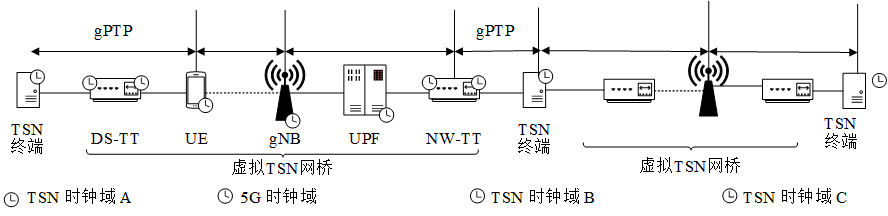
\includegraphics[width=0.95\textwidth]  {fig12.png}} 
	\caption{5G网桥}
\end{figure}
\paragraph{5G网络授时功能}
5G网络现有的时钟同步方案除了卫星授时外,再卫星信号差的应用场景下,会采用1588v2协议进行同步。对于终端设备,5G网络则通过自己定义的广播信息块9(SIB9),以基站广播的方式实现终端之间的时钟同步\textsuperscript{\cite{schungel2021optimized}}。

\paragraph{5G广播同步}


在进行接入终端的时钟同步时,5G网络拥有一套现有的协议流程。第一步为接收端和发射端在时间域和频率域的同步,并不在5G协议的规定范围内。常用方法为互相关检测和自相关检测,通过将接收信号和已知信号PSS作互相关检测检测已知信号的位置,或者对接受信号自身做自相关检测来检测循环前缀CP的位置,获得ofdm符号同步和检测同步信号所在的频率\textsuperscript{\cite{goodarzi2020synchronization}}。
其核心思路即通过基站广播SIB数据包,使得在终端在接入小区的过程中实现一次同步,并在一段时间后进行周期性广播来进行校正以保证精度。
该方法相对1588v2的流程通信开销较小,但由于单向时延测量的原因,其精度只能达到μs级。
\begin{figure}[htb] 
	\center{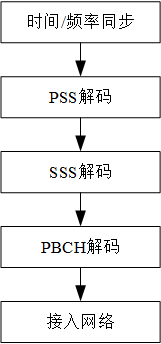
\includegraphics[width=0.5\textwidth]  {fig5.png}} 
	\caption{5G广播同步流程}
\end{figure}
\paragraph{5G与TSN融合同步方案}
现有的5G协议中提供的方案为网桥方案\textsuperscript{\cite{nikhileswar2022traffic}},即利用了1588v2中的透明时钟概念。TSN交换机和用户UE都是与基站gnb进行同步,交换机再接入TSN有线网络。
当要开始进行TSN模式时,即有时间敏感流要通过5G进行传输时,就会通过降低时延来达到高精度的同步要求。
切换到TSN mode的时候需要控制信道,同步的时候为业务信道进行配合,相关信道:synchronization block(SS)   physical broadcast channel(PBCH)
其中值得关注的信号和信道为PSS(primary synchronization signal)和SSS(secondary synchronization signal)。相较于有线网络中的同步,误码率即通信质量也会对同步精度造成影响。
\paragraph{现有的融合优化方案}
对于5G-TSN融合网络,文献\cite{nasrallah2018ultra}提出将5G系统作为TSN桥接器,设计自适应模块来处理TSN协议和信息。 上述方案的优点是5G系统的参数和流程不会暴露给TSN网络。 5G Release 16 协议将上述提议纳入规范,并在 5G 系统的两个边缘引入了新的实体来提供 TSN 转换功能,即 UPF 层的 NW-TT 和终端侧的 DS-TT \textsuperscript{\cite{wang2020leveraging}}。 研究\cite{neumann2018towards}分析了由 5G 和 TSN 网络组成的不同混合拓扑方案,具有不同的特性和用例。 基于此,研究\cite{chai2021cross}提出了一种时钟同步技术,将单向消息机制和 IEEE 802.1AS 相结合,用于 5G-TSN 集成网络,显着降低了同步开销。 对于NW-TT和DS-TT,有研究者\cite{lei20215g}分析了下行链路的时钟同步过程,提出了一种可以支持多个时钟域协同工作的设计方案。 但 5G 时钟域和 TSN 时钟域在同步过程和时序消息方面存在差异。 在5G-TSN融合网络中实现低复杂度和高精度的跨域时钟同步仍然是一个难题。针对该问题,文献\cite{schungel2022time}提出了一种5G-TSN融合网络中基于数据包中继的跨域时钟同步,可以联合估计端到端时钟频率偏移和相位偏移。但是该方案主要关注于基站和TSN设备之间的协调同步,对于无线网络内部的累积误差依然缺少处理。

实际应用过程中,由于5G网络低延迟,高精度的特性,是最有可能成为未来无线TSN载体的通信协议。目前针对5G和TSN融合的问题,3GPP协议和各通信厂商给出的解决方案为5G网桥。通过CNC对5G网络分配网桥的角色,并在有线无线交接处的协议转换器记录时间戳来计算5G网络内部的驻留时间,从而实现5G网络两端的TSN有线设备满足同步要求。但是该方案并不能满足未来无线TSN设备的同步需求,因为其并没有解决无线网络内部的累积同步误差问题,会使得同步精度偏低。

同时,在工业控制系统中,工业通信网络需要高可用性、高可靠性和低延时。然而,传统的工业以太网系统是封闭的,相互之间不兼容(如表1,2所示)。为了提高实时能力,IEEE 802.1时间敏感网络(TSN)标准被广泛认为是工业控制系统中专有技术的长期替代品。此外,工业4.0和未来工厂需要以太网中的无线网络接入。尽管如此,传统的无线网络面临着传输延迟大和距离短的问题(如表所示)。第五代(5G)移动/蜂窝技术,旨在支持超可靠低延迟通信(URLLC),有望满足工业系统在无线领域的严格要求。因此,5G和TSN系统的综合运行对于实现工业网络的端到端确定性连接至关重要。文献\cite{zhang2022wireless}介绍了5G+TSN组合系统在工业现场的应用。
\begin{table}[!htbp]
	\centering
	\caption{目前主要的以太网协议}
	\begin{tabular}{|c| c|c|c|}
\hline
\textbf{协议名称}& \textbf{运作组织}& \textbf{代表厂家} \\
\hline
EtherNet/IP
& ODVA
& Rockwell \\
\hline
PROFINET
& PROFIBUS
& Siemens \\
\hline
EtherCAT
& EtherCAT Association
& Bev \\
\hline
POWERLINK
& EPSG
& ABB \\
\hline
CC-LINK
& CC-Link Association
& Mitsubishi \\
\hline
	\end{tabular}
\end{table}
% 第二个表格
\begin{table}[!htbp]
	\centering
	\caption{目前主要的无线网协议}
	\begin{tabular}{|c| c|c|c|}
\hline
\textbf{协议名称}& \textbf{传输延迟}& \textbf{传输距离} \\
\hline
LTE
& 6ms
& 400-1000m \\
\hline
WIFI
& 6ms
& 100-200m \\
\hline
Zigbee
& 1-3ms
& 10-100m \\
\hline
	\end{tabular}
\end{table}


时钟同步是5G+TSN集成的基础。3GPP协议提出了一种基于IEEE 802.1AS的桥接器架构同步模式,但没有明确指定具体的同步规则和算法细节\textsuperscript{\cite{888888}}。之前的研究\cite{9527833}分析了在同步架构中桥接器和TSN节点交接处可能存在的各种错误对同步算法的影响。研究\cite{9211936}优化了5G桥内的同步数据包,降低了通信开销。另一项研究\cite{9674640}引入了时钟域补偿技术,以估计5G定时消息的驻留时间。

综上所述,目前5G网络对于时钟同步虽然提出了具体的要求,但是还缺乏具体的解决方案,尤其是对于未来高精度的无线时钟同步应用场景,例如以5G为媒介的大规模的无线TSN网络,现有的解决方案往往存在精度较低或者计算过于复杂,同步效率较低的情况。同时,当前的研究仅考虑单个5G桥的最简单情况\cite{9557468},并不能满足在未来的工业和5G网络集成的智能工厂中,多个工业以太网应用场景可能通过时域内的5G网络协同工作\cite{8402373}(图1-4)的情况。
\begin{figure}[htb] 
	\center{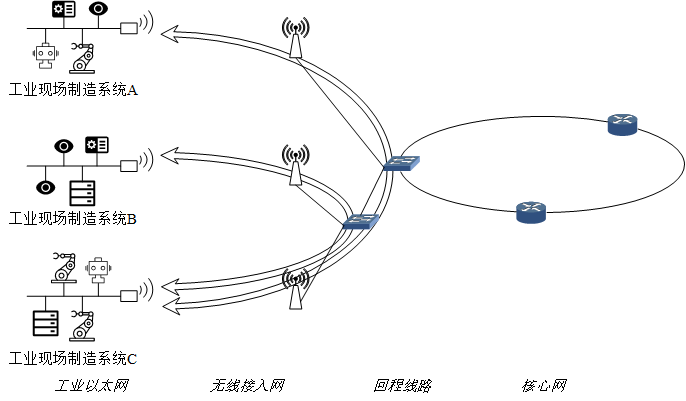
\includegraphics[width=0.95\textwidth]  {fig11.png}} 
	\caption{分布式多领域制造系统应用场景}
\end{figure}

\subsection{本文的研究内容}
根据以上小节,本文总结了三点以5G-TSN为代表的异构网络协同需求:
\begin{itemize}
	\item 全区域最低同步精度应达500ns,以满足未来无线TSN需求
	\item 应尽量避免双向同步和多次重传同步,以减少通信开销
	\item 应补偿无线节点内部的累积误差,以应对大规模无线网络节点场景
\end{itemize}
根据现有的5G-TSN网络的同步需求,本文整理了现有的各种同步方案在各方面的性能,如表1-1所示。
% 第三个表格
\begin{table}[!htbp]
	\centering
	\caption{有线/无线网络同步方案性能总结}
	\begin{tabular}{|c| c|c|c|}
		\hline
\textbf{同步方案}   &\textbf{同步精度}  & \textbf{通信开销}  & \textbf{针对大规模网络的适应性}  \\
\hline
1588v2    & 高   & 大    & 不具备                \\
\hline
广播同步 &  低 &  小 & 具备   \\
\hline
5G网桥 &低   &小     &不具备  \\
\hline
改良后的跨时钟中继网桥同步 &高  & 中        & 不具备    \\
\hline
	\end{tabular}
\end{table}

从表1.3可以看出,现有的异构网络同步方案依然无法完全满足未来5G-TSN融合网络的同步需求。对于传统的1588v2同步而言,虽然具有高精度或者高拓展性的优点,并且机制简单,但其通信开销非常大,包括多次的收发解包,重传确认,校验和周期性重同步。而广播同步虽然拥有良好的可拓展性和较小的通信开销,但其同步精度无法满足TSN对于无线网络的精度需求。5G网桥方案虽然足以应对现有的部分应用场景,但其依然没有解决无线网络内部同步精度较低的问题,无法面向未来的无线TSN需求,改良后的方案则对于大规模的节点所产生的累积误差依然缺少处理。
综合现有的异构网络同步方案的性能和问题,本文提出了一种具有有线骨干网络和多个较小无线岛的混合架构同步方案,以实现有线无线网络节点之间的多节点协同调度。该方案与现有的异构网络时钟太同步方案的主要区别在于,一来无线部分应满足与有线部分相同的同步要求,二来简化无线部分同步步骤,降低无线部分的通信开销,将大规模无线网络节点的累积误差纳入考虑范围内,以此最小化其对于同步精度的影响,从而达到高精度高效率的异构网络时钟同步,实现5G-TSN设备之间跨网络区域协同操作。本文的主要贡献如下:
\begin{itemize}
	\item 提出了新的有线骨干网络和多个较小无线岛的混合架构,并针对其设计了异构同步方案,减少了无线内部同步的累积误差,实现了有线无线网络之间的同步补偿,该方案能应用于大规模无线网络的情况,具有很强的可拓展性和实用性。
	\item 在该同步架构的基础上,本文提出了载波间距优化方案与时间戳补偿方案,以解决同步精度和带宽利用率之间的权衡问题,以及多个网桥存在的情况下的累积误差问题。
	\item 在matlab和omnet上进行了模拟的仿真实验,以验证该方案的可用性,并于现有的方案进行对比,证明其时钟同步的高精度和鲁棒性。
\end{itemize}

\subsection{本章小结}
本章介绍了时钟同步在分布式系统和网络中的重要性,并对有线和无线时钟同步技术的发展和应用进行了探讨。有线网络时钟同步方面,介绍了IEEE 802.1AS协议;无线网络时钟同步方面,介绍了各类用聚类算法。针对有线/无线异构网络时钟同步,介绍了基于网络协议、GPS以及数据融合的时钟同步算法。然而,现有研究在大规模复杂异构网络中的适用性、动态性和可扩展性、安全性和鲁棒性以及满足不同应用场景的特定需求等方面仍存在缺陷。5G和TSN技术在异构网络中的时钟同步显得至关重要,因为它为各种应用场景提供更高的同步精度和更低的同步延迟。结合两者可以实现高效且可靠的时钟同步方案。然而,实现低复杂度和高精度的跨域时钟同步仍然是一个难题。现有解决方案往往存在精度较低或计算过于复杂,同步效率较低的情况。针对有线和无线异构网络中的时钟同步问题,提出了一种以5G-TSN为核心网络的混合架构时钟同步解决方案。

\newpage
\fancyhead[LH]{上海交通大学学位论文}
\fancyhead[RH]{第二章\quad有线/无线网络混合时钟同步架构设计构}
\section{有线/无线网络混合时钟同步架构设计}

本章节将详细介绍时钟模型,时延模型,并以此进行混合同步架构的设计,初始化的同步算法设计,讲解如何提升在大规模异构网络的应用场景下的时钟同步精度和同步效率。

\subsection{时钟模型}
工业现场的复杂性大大影响了设备时钟的晶体振荡器,导致初始时钟状态和变化率的偏差,造成时钟误差。因此,节点时钟表示为::
\begin{equation}
	C_i(t) = (\alpha _i+\sigma_i)t + \beta _i +\delta_i
\end{equation}
其中$\alpha_i$和$\beta_i$是估计的时变时钟偏移和参考时钟的恒定时钟偏移,$\sigma_i$和$\delta_i$是频率估计和时间差的误差。理想情况下,$\alpha_i = 1$,$\beta_i = 0$。斜率的变化来自于时钟内部晶体振荡器的漂移,而初始状态的差异来自于网络初始化期间的误差。

在5G-TSN桥接结构中(如图1-2所示),5G和TSN网络运行在不同的时域。因此,对于目前5G-TSN网络的桥接结构,TSN时域的时钟模型可以表示为:
\begin{equation}
	C_{TSN}(t) = (\alpha_{TSN}+\sigma_{TSN})t + \beta _{TSN} +\delta_{TSN}
\end{equation}
类似地,5G部分的时钟模型写成:
\begin{equation}
	C_{5G}(t) = (\alpha_{5G}+\sigma_{5G})t + \beta _{5G} +\delta_{5G}
\end{equation}
其中$\alpha_{TSN}$和$\sigma_{TSN}$代表有线侧的频率同步校正估计值和误差,$\beta_{TSN}$和$\delta_{TSN}$代表有线侧的时间偏差同步校正估计值和误差。同样,$\alpha_{5G}$和$\sigma_{5G}$代表无线侧的频率同步校正估计值和误差,而$\beta_{5G}$和$\delta_{5G}$代表无线侧的时偏同步校正估计值和误差。

假设同步误差$\sigma_{TSN}$和$\delta_{TSN}$远小于5G网络的$\sigma_{5G}$和$\delta_{5G}$。通常情况下,5G网络的同步精度是微秒级的,而TSN网络的同步精度是纳秒级的。当只有一个网桥时,这些误差通常是可以接受的,但在网络中有多个网桥的情况下,误差的累积会大大影响时钟同步(如图2.1所示)。这些时间戳误差通过影响时钟同步期间的延迟测量而影响同步的准确性。因此,为了减少误差,我们需要对延迟进行建模和分析。
\subsection{时延模型}
在同步过程中,节点之间的延迟是影响同步精度的重要因素。在网桥结构中,5G网桥是由所有5G无线节点中转信号组成的。因此,5G网络内部节点之间的传输延迟决定了网络桥的传输延迟,从而影响两端TSN设备的时钟同步精度。因此,延迟的模型是::
\begin{equation}
	D=D_d+D_r
\end{equation}
其中$D_d$是确定性延迟,主要由可以测量或消除的传输延迟组成。$D_r$是随机延迟,主要由传播延迟抖动和累积误差组成。虽然传播延迟抖动可以定期测量以减少其对同步精度的影响,但累积误差对大规模网络的时钟同步精度有很大影响。为了分析累积误差的具体影响,有必要对排队延迟进行建模。
\begin{figure}[htb] 
	\center{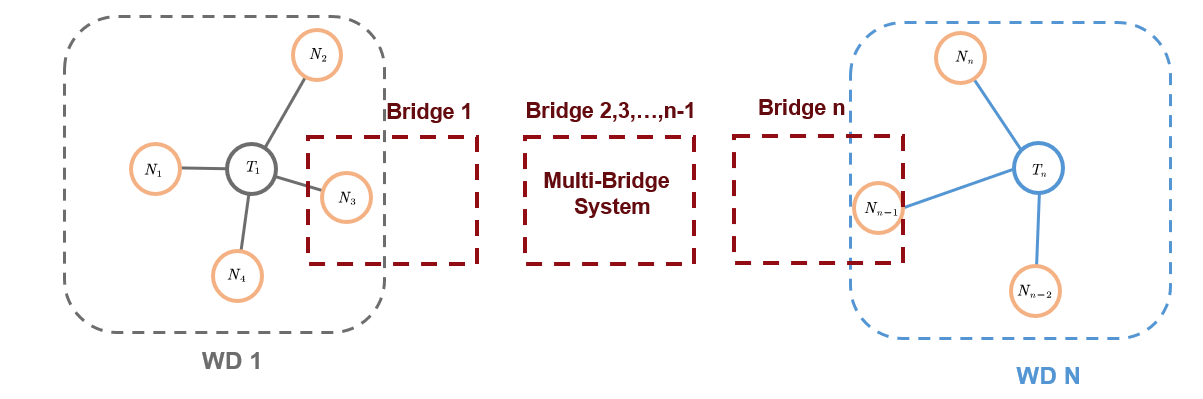
\includegraphics[width=0.95\textwidth]  {fig21.png}} 
	\caption{多网桥场景下的5G内部同步模式}
\end{figure}
5G网络的内部同步模式如图3所示,5G无线节点通过接收基站的同步信息进行同步。当多个节点同时与同一个基站同步时,会出现排队延迟。为了计算排队时延的预期值,首先计算由分批到达交换机的非时钟同步流量产生的队列,通过计算队列的生成函数得到队列的预期值。然后,分析背景流量存在下的时钟同步流量的队列延迟,以获得队列的预期长度。背景流量的计算采用了非抢占式的考虑,这更符合实际情况。对非时钟同步流量队列和时钟同步流量队列都进行了建模,并利用排队理论对马尔可夫链进行建模和求解。根据马尔可夫链列出的稳态方程为:

\begin{equation*}
	p_i\left( \lambda +i \mu \right) =\sum_{j=0}^i{p_j \lambda  a_{i-j}+p_{i+1}\left( i+1 \right)  \mu\, ; 0\leqslant i<m}
\end{equation*}
\begin{equation}
	p_i\left( \lambda +m \mu \right) =\sum_{j=0}^i{p_j \lambda  a_{i-j}+p_{i+1}m \mu}\,; m\leqslant i
\end{equation}
其中$p_i$是$i$数据包在队列中的概率,$m$是队列的最大值,$\lambda$是总的数据包到达率,$\mu$是数据包处理率,$a$是数据包到达数量的分布。而$c=\mu/\lambda $。我们假设当$k$数据包到达基站时,有$v$非时钟同步的数据包。可以有三种情况:
\begin{itemize}
	\item 1: $v<m$, $k<m-v$, QueueLength = 0。
	\item 2: $v<m$, $k>m-v$, QueueLength = $k+v-m$.
	\item 3: $v>m$, QueueLength = $k$.
\end{itemize}

基于这三种情况,排队延迟的期望值可以通过求解马尔科夫链和用全概率公式求和来获得。
\begin{equation*}
	L_q=P_0 \sum_{i=0}^m{\left(k-m+i\right) \frac{\left(\lambda/\mu\right)^i}{i!}+P_0 \frac{k-m}{m!} \frac{\rho^m}{v!\left(1-\rho^m\right)}}
\end{equation*}
\begin{equation}
	\rho=\frac{\lambda}{\mu}
\end{equation}
根据5G协议标准3GPP TS 22.104对大规模应用场景的要求,当服务区域在10到20$km^2$之间时,单个时域的同步节点的上限为100\textsuperscript{\cite{888889}}。通过将这些条件代入排队延迟模型,可以得到排队延迟小于250ns。鉴于所要求的同步精度为1$\mu s$,随机排队延迟对同步精度的影响可以忽略不计,只有固定延迟影响同步精度。因此,我们对多场制造系统方案的时间戳补偿只关注这些条件下固定延迟对时钟同步的影响。

\subsection{混合同步架构设计}

混合同步架构是一种专门针对大规模异构网络场景设计的同步方法,在大规模的异构网络协同中有着良好的性能优化,能最小化传输开销,累积误差以及时序误差。如图2-4所示,混合同步架构由有线骨干网络和多个较小无线岛组成。上层核心网络部分由5G+TSN节点组成,下层网络由各种工业以太网和无线传感器组成。上层核心网络建立高精度5G+TSN时钟同步后,架构内会选取边界节点,下层网络将作为从时钟,根据自己的同步需求与边界节点进行同步。

为了将异构网络中混乱的网络分层整合起来,本发明提出了一种基于混合同步架构的t同步方法。最上层主干网络是5G+TSN,中下层包括各种网络,如工业以太网、Wi-Fi、Zigbee、LoRaWAN、Bluetooth等。在整合这些网络时,需要参考前面得到的参数。为了更加具体地根据时钟稳定性、排队延迟和累计误差等因素进行划分,并设计一个综合指标来评估不同区域网络属于哪个层级。这样,我们可以更精确地将具有相似特性的网络划分到同一层级,以便采用合适的同步策略和优化方法。
针对这个需求,我们可以引入一个名为“网络同步性能指标(NSPI)”的综合评估指标。

NSPI 可以综合考虑时钟稳定性、排队延迟和累计误差等因素,并为每个区域网络分配一个NSPI值。我们可以根据NSPI值的范围来确定网络属于哪个层级。例如,设定不同层级对应的NSPI值范围如下:
\begin{itemize}
	\item m1层级:NSPI值在A1-A2范围内
	\item m2层级:NSPI值在B1-B2范围内
	\item ...
	\item mn层级:NSPI值在Z1-Z2范围内
\end{itemize}

根据我们的分层目的,我们希望确保网络能够根据同步精度需求以及各自的性能特点井然有序地进行时钟同步。为了避免低精度要求但性能较差的网络被分到高层级,我们可以对NSPI值计算公式进行进一步改进。可以考虑将SPW因子用于调整各项参数的权重,而不是直接乘以NSPI值。新的NSPI值计算公式如下:
\begin{equation}
	NSPI = (W1 * SPW * \delta) + (W2 * (1 - SPW) * (n * \beta * (1 + p) / \mu)) + (W3 * D_{\text{RMSE}})
\end{equation}

这里,当SPW越接近1时,$\delta$项(时钟稳定性)的权重增加,而排队延迟项(n * $\beta$ * (1 + p) / $\mu$)的权重减小。这样,具有高同步精度需求的网络将更加注重时钟稳定性。相反,当SPW越接近0时,排队延迟项的权重增加,而时钟稳定性项的权重减小。这样,具有低同步精度需求的网络将更加注重处理能力和网络规模。
通过调整SPW的值,我们可以确保网络根据其同步精度需求和性能特点进行分层,从而实现复杂异构网络的井然有序时钟同步。在实际应用中,可以根据不同网络的同步精度需求和性能特点,对混合同步架构进行进一步优化。
分层过程如图2-4所示:

\begin{figure}[htb]
	\center{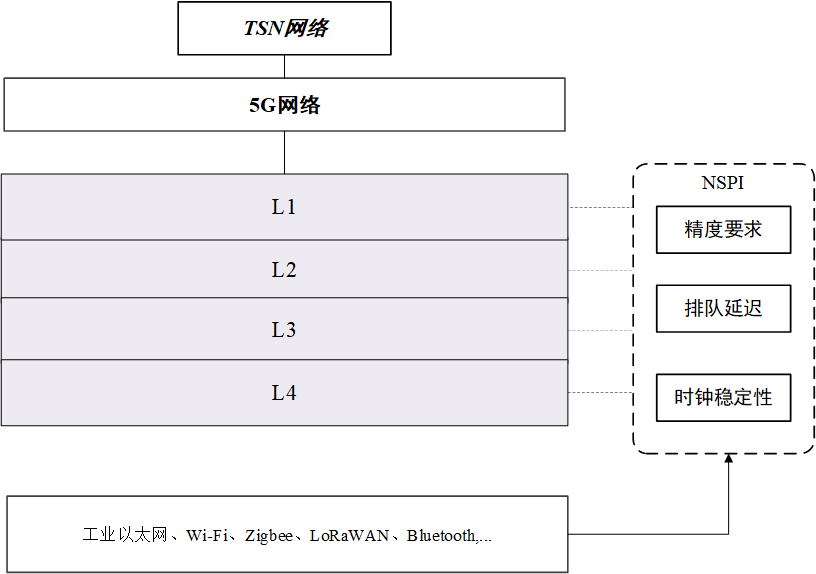
\includegraphics[width=0.95\textwidth]  {fig29.png}}
	\caption{\label{1} 混合架构分层过程}
\end{figure}

另外在分层过程中,需要注意不能改变原有网络拓扑结构中的连接关系,分层的本质是通过链路选择来使得每一层的网络能选择最优的同步对象。
整体分层算法如算法1所示,下面将详细阐述分层算法的流程:
\begin{algorithm}
	\caption{分层算法}
	\begin{algorithmic}[1]
		\STATE 对图 $G=(V,E)$ 进行预处理
		\STATE 定义权重函数 $w(u, v) = \alpha d(u, v) + \beta j(u, v)$
		\STATE 构建最小生成树:使用 Kruskal 或 Prim 算法
		\STATE 初始化生成树 $T$
		\STATE 选择顶层 TSN 节点 $r \in V_T$ 作为根节点
		\STATE 分层:进行深度优先搜索(DFS)或广度优先搜索(BFS)
		\STATE 初始化层级 $L(r) = 1$
		\STATE 遍历生成树,分配层级 $L(v) = L(u) + 1$,其中 $(u, v)$ 是树中的边
		\STATE 分析与优化:计算平均同步延迟 $\bar{d}$ 和抖动 $\bar{j}$
		\STATE $\bar{d} = \frac{1}{\lvert E' \rvert} \sum_{(u,v) \in E'} d(u,v)$
		\STATE $\bar{j} = \frac{1}{\lvert E' \rvert} \sum_{(u,v) \in E'} j(u,v)$
		\STATE 如果需要,优化分层结构,例如调整阈值 $T$ 或添加额外约束条件
	\end{algorithmic}
\end{algorithm}

我们可以将问题建模为一个有向图G=(V, E),其中V表示网络节点集合,E表示节点之间的连接,然后采用下述方法进行:
\paragraph{预处理}对图 $G=(V,E)$ 进行预处理,其中 $V$ 是节点集合,$E$ 是边集合。我们将同步性能指标(例如,传播延迟 $d$、抖动 $j$ 等)作为边的权重。对于边 $(u, v) \in E$,我们可以定义权重函数 $w(u, v) = \alpha d(u, v) + \beta j(u, v)$,其中 $\alpha$ 和 $\beta$ 是权重系数。

\paragraph{构建最小生成树}使用 Kruskal 或 Prim 算法从顶层 TSN 节点开始构建一个最小生成树。假设 $V_T \subseteq V$ 是顶层 TSN 节点集合,我们可以从任意顶层节点 $r \in V_T$ 开始构建最小生成树。对于 Kruskal 算法,我们需要对所有边按权重排序,即对于任意边 $(u, v), (u', v') \in E$,有 $w(u, v) \le w(u', v')$。然后,从最小权重边开始,依次添加边到生成树中,直到所有节点都被连接。在添加边的过程中,我们需要确保不会产生环。对于 Prim 算法,我们从根节点 $r$ 开始,每次添加距离当前生成树最近的边,直到所有节点都被连接。

\paragraph{分层}从最小生成树的根(即顶层 TSN 节点)开始,进行深度优先搜索(DFS)或广度优先搜索(BFS)。在遍历过程中,根据节点在树中的深度和NSPI值为其分配层级。设 $L(v)$ 是节点 $v$ 的层级,则有 $L(r) = 1$。对于节点 $u$ 的邻接节点 $v$,有 $L(v) = L(u) + 1$。

\paragraph{分析与优化}:根据生成的最小生成树和分层信息,分析网络的同步性能。我们可以计算各层间的平均同步延迟 $\bar{d}$ 和抖动 $\bar{j}$,例如:
\begin{equation}
	\left\{
	\begin{aligned}
			\bar{d} = \frac{1}{\lvert E' \rvert} \sum_{(u,v) \in E'} d(u,v),\\
		\bar{j} = \frac{1}{\lvert E' \rvert} \sum_{(u,v) \in E'} j(u,v)
	\end{aligned}
	\right.
\end{equation}
其中 $E'$ 是最小生成树的边集合。如果需要,可以进一步优化分层结构,例如调整阈值 $T$ 或添加额外的约束条件。这可以通过修改权重函数 $w(u, v)$ 和调整搜索过程来实现。

通过这种方法,我们可以将原始的拓扑结构分层,使得每个节点只能通过一条路径向上同步,从而减少同步过程中的混乱。详细分析如下:
我们假设我们有一个网络拓扑图$G(V, E)$,其中$V$表示节点集合,$E$表示边集合。我们定义出错概率$P(e)$为一条边$e$的出错概率。为简化问题,我们假设所有边的出错概率相同,即$P(e) = p (0 < p < 1)$。

令$d(u, v)$表示节点$u$和$v$之间的最短路径长度。在网络同步过程中,信息沿着边从一个节点传播到另一个节点。给定一条从节点$u$到节点$v$的路径$P(u, v)$,我们可以计算这条路径的可靠性$R(P(u, v))$。如果路径$P(u, v)$包含$k$条边,则$R(P(u, v))$表示$k$条边都没有出错的概率,即:

\begin{equation}
	R(P(u, v)) = (1 - p)^{d(u,v)}
\end{equation}

在分层结构中,节点之间的同步路径被限制在相邻层次之间。设分层后的网络拓扑为$G'(V, E')$。我们定义两个网络的可靠性分别为:

\begin{equation}
	R(G) = \sum_{u, v \in V} R(P(u, v))
\end{equation}

\begin{equation}
	R(G') = \sum_{u, v \in V} R(P'(u, v))
\end{equation}

我们的目标是证明$R(G') \ge R(G)$。为了简化问题,我们可以考虑节点对$(u, v)$之间的可靠性差异$\Delta R(u, v) = R(P'(u, v)) - R(P(u, v))$。如果对于所有节点对$(u, v)$,我们都有$\Delta R(u, v) \ge 0$,那么我们就可以得出结论$R(G') \ge R(G)$。

\begin{equation}
	\Delta R(u, v) = (1 - p)^{d'(u,v)} - (1 - p)^{d(u,v)}
\end{equation}

其中,$d'(u,v)$表示分层后节点$u$和$v$之间的最短路径长度。

由于分层结构限制了同步路径仅在相邻层次之间,我们可以推测$d'(u,v) \le d(u,v)$。如果这一推测成立,那么对于所有节点对$(u, v)$,我们有:

\begin{equation}
	\Delta R(u, v) = (1 - p)^{d'(u,v)} - (1 - p)^{d(u,v)} \ge 0
\end{equation}
从而可以证明$R(G') \ge R(G)$。
总之,分层后的网络结构有以下优势:
\begin{itemize}
	\item 提高同步效率:在分层结构中,每个节点都有明确的同步路径,可以减少同步过程中的冗余和冲突,提高同步效率。
	\item 降低同步延迟和抖动:分层结构可以使得每个节点在同步过程中遵循最短路径,从而降低总体的同步延迟和抖动。
	\item 易于管理和优化:分层结构使得网络变得更加清晰和简洁,便于分析和优化网络性能。例如,我们可以针对不同层级的节点采取不同的同步策略,以适应不同场景和需求。
\end{itemize}

总之,通过引入图论和搜索算法,我们可以将原始的网络拓扑分层,使得每个节点在同步过程中遵循唯一路径,从而提高同步效率和降低同步延迟与抖动。这种方法可以广泛应用于具有多个节点和复杂连接关系的网络系统,为实现高效、稳定的网络同步提供了一种有效的解决方案。


在完成分层后,网络结构将会如图2-5所示。此时网络可以分为上层的核心网络与下层的其他网络。上层的核心网络中为5G网络与TSN网络,下层网络内部将根据规则氛围若干层级,按照低层级向高层级的规则进行同步。同步周期可以如下图表示:

\begin{figure}[htb]
	\center{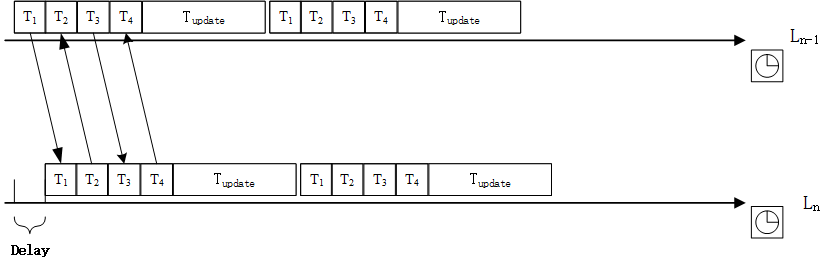
\includegraphics[width=0.95\textwidth]  {fig30.png}}
	\caption{\label{1} 混合同步架构}
\end{figure}
如图所示,每个层级之间的一个工作周期周期包括同步周期与一个校验更新周期。在同步周期内下层将会与上层进行时间戳交互并完成参数计算。由于下层网络与上层网络非对称同步的特性,尤其是对于下层中的无线传感器网络,其节点对于时间戳计算中涉及到的浮点数计算精度不足,因此在同步过程中,涉及到边界补偿的时间戳的计算都将在核心网络进行,然后通过下行链路传输到下层网络,可以有效利用核心网络中TSN节点的计算资源,提高同步效率,同时也是为了提升整个异构网络的同步精度。而在校验更新周期内网络将对拓扑结构,时钟参数进行校验,以防止外界因素影响时钟同步精度。
该架构将基于工业以太网网络的不同岛屿区域制定为相应的时域模型。5G网络作为这些有线岛屿之间的桥梁。在3GPP中,在集成的5G和TSN系统中考虑了两个主要的时钟模型用于时间同步,这两个模型都符合IEEE 802.1 AS标准。这些模型包括边界时钟和透明时钟\cite{9615318}.

在边界时钟中,5G无线接入网(RAN)可以直接访问TSN主时钟,通过自己的信令和程序向用户设备(UE)提供定时信息。UE根据周期性信息来同步TSN设备。相比之下,透明时钟解决方案通过交换PTP信息实现时间同步。在TSN主控台和TSN设备之间的任何中间5G或TSN实体将通过实体中的新PTP消息更新时间。

5G网络作为透明时钟,而有线网络作为边界节点。5G RAN可以直接访问TSN主时间,可以通过直接连接TSN主时钟或通过支持PTP的底层传输网络,这可以减少5G网络中TSN时间戳的传输开销。

为了满足假设和通信协议,每个网桥的无线节点数量不应超过100。当节点数量超过这个数字时,将建立一个新的边界节点来分割网络桥。图2.4显示了整体架构图。

\begin{figure}[htb]
	\center{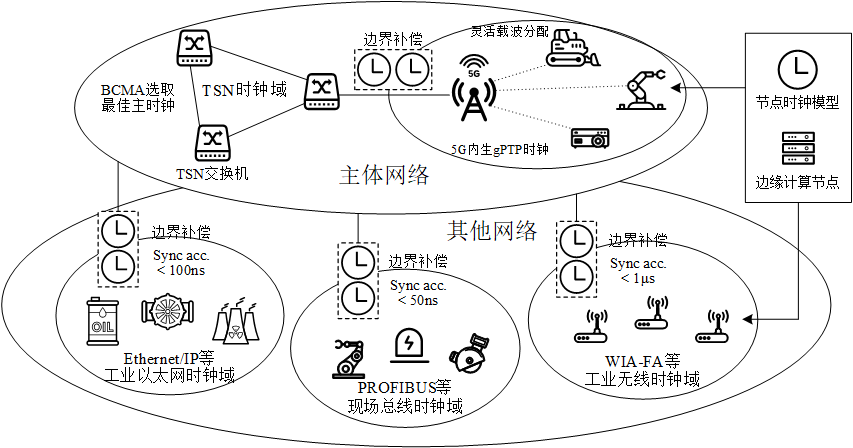
\includegraphics[width=0.95\textwidth]  {fig17.png}}
	\caption{\label{1} 混合同步架构}
\end{figure}

\subsection{初始化同步}

在此阶段,有线无线网络先分别进行各自的初始化同步。有线网络通过自带的802.1AS进行同步,无线网络则通过广播方式进行单向同步,其内容包括节点接入,拓扑确认,层级编号以及主从时钟定位。这些参数将被用于确定后续的同步操作,即累积误差补偿和边界补偿。后续阶段的误差补偿都是分层级完成的,没个层级都存在自己的主从时钟配对,配对方式由上文中的参数决定。
\subsubsection{有线部分初始化同步}

有线部分的初始化同步采取gptp同步方案,IEEE 802.1AS 规定了用于 TSN 网络中时间同步的 gPTP。 它定义了传播延迟测量以及频率和时间同步的机制。 gPTP 定义了两种类型的时间感知系统 (TAS),它们是时间感知终端站 (TAE) 和时间感知桥 (TAB)。 TAS 可以是从属实体或主实体。 每个时域只有一个主实体。 此外,在 gPTP 范围内称为大师 (GM) 的主实体充当时间感知网络 (TAN) 内所有从属实体的参考时间源。 TAN 与一个或多个时域相关联。 因此,TAS 可以同时成为不同时域的成员。
时钟偏差补偿方案采用上文中(1.1)的IEEE 1588v2协议中的方式进行计算:
\begin{equation}
	D = \frac{((t_2-t_1)+(t_4-t_3))}{2} 
\end{equation}
\subsubsection{无线部分初始化同步}
为了实现有线部分的同步,我们采用了GPTP同步方案,因此混合架构中的无线网络部分可以视为gptp中的一个单独的时域存在,而基站则作为其GM而存在,广播同步则完成了无线部分的同步。当时间戳通过透明时钟时,5G网桥内的同步精度会影响时间计算的精度。为了同步5G-TSN网桥内的多跳大规模无线网络节点的时钟,我们首先需要确定每个节点的层次结构,这也是定位每个无线节点的基础。

根节点以$k=0$的计数发起同步消息,接收节点将计数设为$k+1$,并将包含$k+1$的广播同步消息发送到下一级,以此类推。直到所有节点都确定自己的级别,并从上至下依次进行同步,如图所示。
\begin{figure}[htb]
	\center{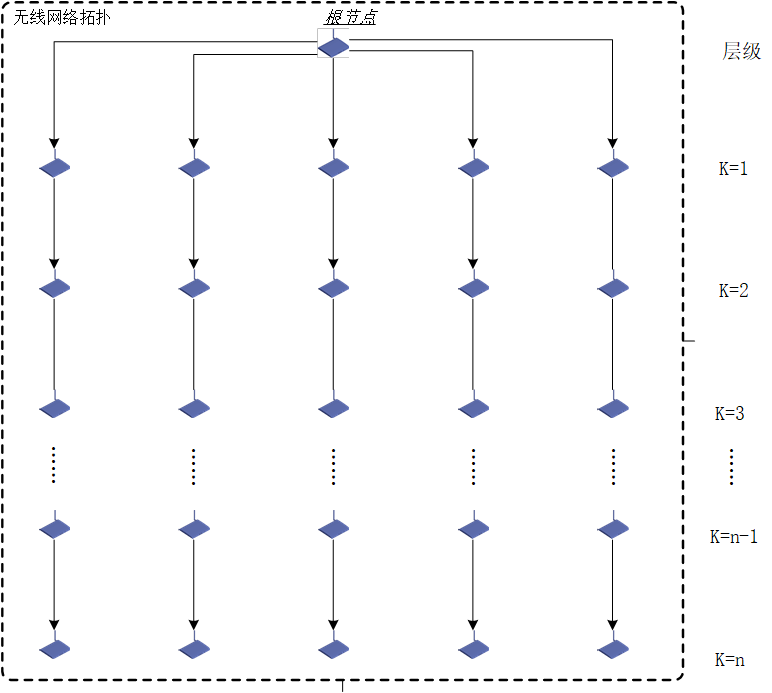
\includegraphics[width=0.95\textwidth]  {fig8.png}}
	\caption{\label{1} 广播同步}
\end{figure}


初始同步按照单向同步方案进行,收到广播的时钟根据解包内的时间戳信息和接收时间直接计算传输延时并对本地时钟进行校正。为了在保持同步精度的同时最大限度地减少能耗和降低计算复杂度,我们针对TSN+5G网络的非对称网络时钟同步特性,采用了反同步的机制\cite{8935413}。时间戳转换涉及浮点除法,由于TSN拥有更多的计算资源,所以需要在TSN端进行。

具体来说,5G节点会定期向两端的边缘节点的TSN开关发起同步请求消息。从属时钟通过几个中间时钟接收来自主时钟的参考时间戳$G$,并记录本地时间$L$,然后将其发送给TSN节点。TSN节点执行一个线性回归过程,通过交换几个时间戳来估计频率差和时钟偏差。中间转发节点被视为一个透明的时钟。无线部分整体的初始化阶段的同步算法2所示。
\begin{algorithm}[ht]  
	\caption{无线网络初始化阶段的时钟同步流程}  
	\begin{algorithmic}[1]
		\REQUIRE GM发送的时间戳, $T_m^1$ and $T_m^2$,$\cdots$, $T_m^n$; 本地节点S记录的时间戳, $T_s^1$ and $T_s^2$,$\cdots$, $T_s^n$; 中央控制系统(CNC)下发的同步精度需求, $prec$;
		\ENSURE 本地的修正时间, $L'$;
		\WHILE {$time \in T_{begin}$}
		\WHILE {$time = nt_slot, n=1,2\ldots $}
		\IF {$prec \geq 500ns$}
		\STATE GM 和无线从节点交换信息, 从节点得到 $T_s^1$ 和 $T_s^2$; 
		\STATE S 计算修正量 $\Delta = [(T_s^1 - T_m^1) - (T_m^2 - T_s^2)]/2$;
		\ELSE  
		\STATE GM 和无线从节点交换信息, 从节点得到 $T_m^1$ and $T_m^2$,$\cdots$, $T_m^n$,通过本地线性回归得到偏差和频率的估计值$\sigma$和$o$	
		\STATE S计算修正量$\widehat{L}=L(1+\frac{\widehat{\sigma}}{f_0})-\widehat{o}+[\frac{G_0-L_0}{T_slot}]T_{slot}$			
		\ENDIF
		\STATE S将层级和修正量参数返回至CNC,等待下一步操作;
		\ENDWHILE
		\ENDWHILE
		%\RETURN $T_{SM}'$.
	\end{algorithmic}
\end{algorithm}

最后,每个无线节点的校正时间被建模为:
\begin{equation}
	\widehat{L}=L\left(1+\frac{\widehat{\alpha}}{f_0}\right)-\widehat{\beta}+\left[\frac{G_0-L_0}{T_c}\right] T_c
\end{equation}
其中$\widehat{α}$代表频率差的估计,$\widehat{β}$是时钟偏差的估计。$[\frac{G_0-L_0}{T_c}]T_c$这一项表示从5G网络节点到TSN节点的传输延迟,$T_c$是5G网络的时隙,是5G-TSN时钟同步期间通过估计传输延迟可以达到的精度上限。这构成了后续同步精度优化方案的基础。

因此混合架构中的无线网络部分可以视为gptp中的一个单独的时域存在,而基站则作为其GM而存在。无线部分的初始化同步则通过广播同步完成,根节点将计数k=0嵌入同步报文广播发送,接收到的节点将计数k进行k+1设定为本地级别并向下一级发送包含k+1的广播同步报文。以此类推。直到所有节点都确定自己的级别,并从上至下依次进行同步。初始同步按照单向同步方案进行,收到广播的时钟根据解包内的时间戳信息和接收时间直接计算传输延时并对本地时钟进行校正。

\subsubsection{校验更新}
在完成累积误差补偿后,混合架构已经完成了有线部分和无线部分的分时域同步。在初始化同步阶段之后,CNC确定了网络拓扑结构以及各节点的层级。然而,工业现场中可能出现的设备节点变动,使得网络拓扑可能随时改变。因此,混合架构需要定期对网络参数进行更新和校验。更新校验的整体算法如算法3所示。
\begin{algorithm}
	\caption{校验更新算法}
	\begin{algorithmic}[1]
		\REQUIRE
		原有网络拓扑,网络参数,节点信息
		\ENSURE
		更新后的网络参数
		\STATE 初始化新增局域网络
		\FOR{每个新增节点 $j$}
		\STATE 选择最近的无线节点作为局域主时钟
		\STATE 采用同步优化规则对节点 $j$ 进行同步
		\ENDFOR
		\STATE 计算中间结果 $M_{ij} = \{(\Delta f_{ij}, \Delta t_{ij})\}$
		\FOR{每个需要进行全局校验的节点 $j$}
		\STATE 更新频偏:$f_j^{new} = f_j + \sum_{i} \Delta f_{ij}$
		\STATE 更新时偏:$t_j^{new} = t_j + \sum_{i} \Delta t_{ij}$
		\ENDFOR
		\STATE 返回更新后的网络参数
	\end{algorithmic}
\end{algorithm}
首先,进行网络拓扑的校验更新。原有的网络节点在后续的网络拓展中无需进行更新,因为网络拓展没有破坏它们原有的主从关系链。原有的网络拓扑同步规则将保留,以节省传输资源。对于新增的网络节点,我们需要更新其本地校验。设新增的无线终端节点集合为 $N_{new}$,由于新增的无线终端节点分布的不确定性,如果直接取与有线主时钟的主从关系,势必要从其他的原有节点中取得原有的网络参数值,从而带来更多的跨机传输开销。因此,选择将其作为一个新增的局域网络,与就近的无线节点 $n_i$ 进行同步。设对接的无线节点 $n_i$ 为之前混合架构中的高精度有线主时钟,采用之前的同步优化规则对新增节点进行同步。这样可以有效节省计算开销,并且由于原有无线节点已经进行过累积误差优化,这样所带来的误差在可接受的范围内。

接下来进行全局校验的生成。设节点 $n_j$ 的频偏和时偏估计值为 $f_j$ 和 $t_j$。当原有拓扑网络节点的离线或故障,或者当同步精度漂移较大时(例如,$|f_j - f_i| > \epsilon_f$ 或 $|t_j - t_i| > \epsilon_t$,其中 $\epsilon_f$ 和 $\epsilon_t$ 是给定的阈值),则需要对原有架构参数进行更新,重新计算频偏和时偏的估计值。

全局校验更新需要从其他节点中获取数据,会产生较大的传输开销。为了降低全局校验更新带来的跨节点传输开销,混合架构可以在结构内优先进行数据的计算,生成一些中间结果 $M_{ij}$,最后只将这些中间结果传输至出现同步问题需要进行全局校验的节点。这些中间结果能够代替原始数据完成校验的运算,保证了校验更新的正确性,并且相较于原始数据,中间结果能够将多个数据块运算成一个数据块,节省了跨节点传输的开销。

具体而言,中间结果 $M_{ij}$ 可以通过在局部范围内计算频偏和时偏的累积变化而生成。对于每个节点 $n_i$,我们可以计算其与邻近节点 $n_j$ 的频偏和时偏变化 $\Delta f_{ij}$ 和 $\Delta t_{ij}$。在这种情况下,中间结果 $M_{ij}$ 可以表示为:
\begin{equation}
	M_{ij} = \{(\Delta f_{ij}, \Delta t_{ij})\}
\end{equation}
当需要进行全局校验更新时,只需将 $M_{ij}$ 传输至出现同步问题的节点 $n_j$。节点 $n_j$ 可以使用这些中间结果来计算新的频偏和时偏估计值:
\begin{equation}
	\left\{
	\begin{aligned}
	f_j^{new} &= f_j + \sum_{i} \Delta f_{ij},\\
	t_j^{new} &= t_j + \sum_{i} \Delta t_{ij}
	\end{aligned}
	\right.
\end{equation}


\subsection{混合架构时钟同步评估指标}

在混合时钟同步完成后,需要对同步效果进行评估,以便根据结果修改同步策略。在异构网络时钟同步领域,主要关注以下几个评价指标\textsuperscript{\cite{chi2018ear}}:
	\paragraph{同步精度}指网络节点之间的时钟偏差,通常使用均方根误差(Root Mean Square Error, RMSE)来度量,定义为:
	\begin{equation}
		D_\text{RMSE} = \sqrt{\frac{1}{N} \sum_{i=1}^{N} (\delta t_{i} - \delta t_{ref})^2}
	\end{equation}
其中,$N$ 是网络节点数量,$\delta t_{i}$ 是节点 $i$的时钟偏差,$\delta t_{ref}$ 是参考时钟偏差。
\paragraph{同步稳定性}指网络节点时钟偏差随时间的变化情况,主要反映时钟同步系统的抗干扰能力。通常使用最大时间间隔误差(Maximum Time Interval Error,MTIE)来度量,定义为:
\begin{equation}
	T_\text{MTIE}(\tau) = \max_{0 \leq t \leq T - \tau} \left\{ \max_{t \leq t' \leq t + \tau} \delta t_{t'} - \min_{t \leq t' \leq t + \tau} \delta t_{t'} \right\}
\end{equation}
其中,$\tau$ 是观察时间间隔,$T$ 是总观察时间,$\delta t_{t'}$ 是时刻 $t'$ 的时钟偏差。
\paragraph{收敛速度}指网络节点时钟同步过程中,达到稳定状态所需的时间,通常使用同步迭代次数来度量。设第 $k$ 次迭代后的同步误差为 $E_k$,同步误差的收敛速度可以定义为:
	\begin{equation}
		v_\text{Convergence} = \min \left\{ k \in \mathbb{N} : |E_k - E_{k-1}| < \epsilon \right\}
	\end{equation}
	其中,$\epsilon$ 是给定的收敛阈值。
\paragraph{能耗}指时钟同步过程中消耗的能源,主要关注无线网络节点的通信和计算能耗。能耗可以定义为:
	\begin{equation}
		E_\text{total}= E_{comm} + E_{comp}
	\end{equation}
	其中,$E_{comm}$ 和 $E_{comp}$ 分别表示通信能耗和计算能耗。
\subsection{性能优化方法}

为了提高异构网络时钟同步的性能,研究者提出了多种优化方法:

\begin{itemize}
	\item 优化报文传输策略:通过调整报文传输的时间间隔、优先级等参数,降低网络拥塞和延时波动对时钟同步的影响\textsuperscript{\cite{mizrahi2012slave}}。例如,可以使用分散优先级的报文传输策略,将报文按照优先级划分为不同的队列,优先传输高优先级的报文,从而降低时钟同步误差。
	\item 自适应同步算法:根据网络状况和节点性能动态调整同步策略,提高同步精度和稳定性\textsuperscript{\cite{fradkov1997adaptive}}。例如,可以设计一个自适应权重系数的同步算法,通过实时监测网络负载和节点状态
	,动态调整有线网络和无线网络时钟同步结果的权重,实现更高精度的时钟同步。
	
	\begin{equation}
		\alpha_{k+1} = \alpha_k + \gamma \cdot \frac{\partial D_\text{RMSE}}{\partial \alpha} (\delta t_{ij}^{(w)}, \delta t_{ij}^{(l)}, \alpha_k)
	\end{equation}
	
	其中,$\alpha_{k+1}$ 和 $\alpha_k$ 分别表示第 $k+1$ 次和第 $k$ 次迭代的权重系数,$\gamma$ 是学习率,$\frac{\partial D_\text{RMSE}}{\partial \alpha}$ 是关于权重系数的同步误差梯度。
	
	\item 优化时钟同步过程中的能源消耗:为了降低能耗,可以采取调整报文传输策略、减少计算量等措施\textsuperscript{\cite{xue2021wicsync}}。例如,在无线网络节点中,可以根据节点的剩余能量动态调整时钟同步的频率,降低能耗。
	
	\item 针对不同应用场景的定制化同步策略:根据异构网络中不同应用场景的特点,设计针对性的时钟同步解决方案,提高同步性能和实用性~\cite{19}。例如,在工业物联网场景中,可以利用工业控制器提供的确定性通信机制,实现高精度和低延时的时钟同步。
	
\end{itemize}




\subsection{本章小结}
本章介绍了一种有线/无线网络混合时钟同步架构设计。首先讨论了时钟模型、时延模型,为了整合异构网络,引入了名为“网络同步性能指标(NSPI)”的综合评估指标,用于网络分层。分层算法将问题建模为有向图,采用预处理方法进行处理,实现井然有序的时钟同步。完成分层后,可以根据最小生成树和分层信息分析网络的同步性能,并在需要时进行优化。分层结构可提高同步效率,降低同步延迟和抖动。接着给出了初始化阶段的同步方案,有线无线网络分别进行各自的同步。有线部分采用gPTP同步方案,无线部分通过广播同步完成。初始同步采用单向同步方案,由于工业现场中设备节点可能变动,网络拓扑可能随时改变,混合架构需要定期对网络参数进行更新和校验。

最后讨论了混合架构时钟同步评估指标,包括同步精度、同步稳定性、收敛速度和能耗等。这些评估指标和优化方法有助于改善时钟同步策略,使之更加高效和可靠。

\newpage
\fancyhead[LH]{上海交通大学学位论文}
\fancyhead[RH]{第三章\quad5G+TSN异构网络的混合时钟同步方法}
\section{5G+TSN异构网络的混合时钟同步方法}
在上一章中,为了解决多场制造系统的场景,我们设计了一个异构网络的同步架构(图2.4),并实现了整个架构的初始化同步以及网络拓扑的校验更新。接下来,我们将针对核心网内部的5G+TSN网络部分进行子载波间隔优化和时间戳补偿,以保证核心网络的同步精度。

\subsection{子载波间隔优化问题构建}
根据公式(2.15),已知5G网络中5G-TSN同步时估计传输延迟的误差上限为$T_c/2$。如图5所示,5G网络的帧结构由一个无线帧和一个相同长度的子帧组成,分别为10ms和1ms。5G的每个时隙包含14个OFDM符号,其中4个 OFDM符号被SSBS(时钟同步信息)占用。SSBS的持续时间和周期随不同的子载波间隔而变化,而5G的子载波间隔可以调整。通过利用子载波间隔的特性,可以通过增加子载波间隔来减少OFDM的子载波数量和符号长度,从而减少延迟和累积误差。因此,我们可以得到 :
\begin{equation}
	\left\{
	\begin{aligned}
		T_{c}&=\frac{15kHz}{\triangle F},\\
		\triangle F&=2^\mu\cdot15kHz.\\
	\end{aligned}
	\right.
\end{equation}
其中$\triangle F$是子载波间距(SCS),$\mu=\{0,1,2,3,4,5\}$。它表明,当有源载波带宽$f_c$固定时,增加子载波间距$\triangle F$可减少时钟同步误差$\varepsilon$。然而,增加载波间距也会引起以下问题:
\begin{itemize}
	\item 频谱效率降低:载波间隔越大,每个载波可传输的数据量就越小,频谱效率也就越低。
	
	\item 抗干扰能力下降:载波间隔越大,遇到干扰源时,误码率越大。
	
	\item 功耗增加:如果要保证低误码率,就需要提高信号功率,这就导致了功耗的增加。
	
	\item 浪费资源:大的载波间隔可能会导致一些频谱资源被浪费掉。
\end{itemize}
选择一个合适的载波间隔对于实现高精度的5G+TSN同步至关重要。这个问题可以简化为同步精度和带宽利用率之间的权衡,可以表示为:
\begin{equation}
	\eta=f_c\cdot \frac{B}{12\cdot N_{RB}\cdot \triangle F}
\end{equation}
其中$N_{RB}$是RB的数量,$B$是网络的带宽。为了找到最佳载波间隔,构建了一个优化问题如下:
\begin{equation}
	\begin{split}
		&\min_{\triangle F} \,\, \omega_1 \cdot T_c+\omega_2 \cdot \frac{1}{\eta} \\
		&s.t.\quad  \left\{\begin{array}{lc}
			T_{cmin}\leq T_c \leq T_{cmax}\\
			B_{min}\leq B \leq B_{max}\\
			N_{RB}\leq 273\\
		\end{array}\right.
	\end{split}
\end{equation}
其中$\omega_1$和$\omega_2$分别代表同步精度和带宽利用率的权重。用户根据自己的需要确定权重。这种方法在不显著影响5G网络通信质量的情况下,将同步误差降到最低。
\begin{figure}[htb] 
	\center{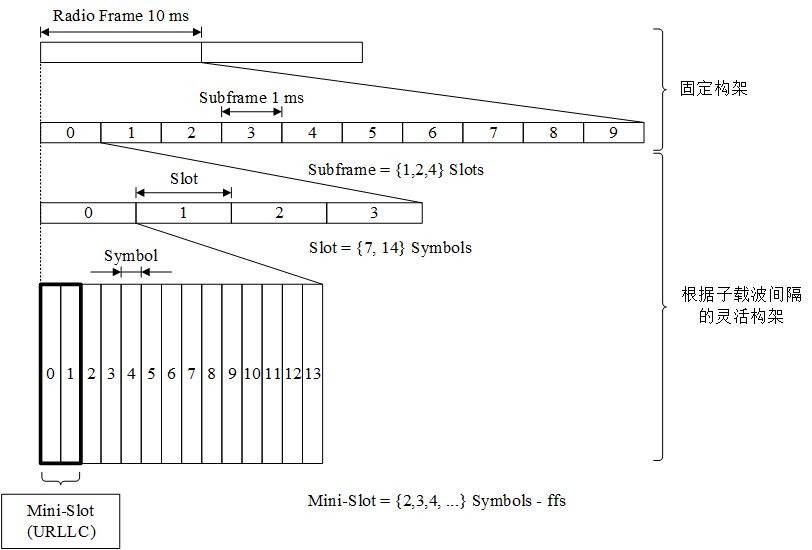
\includegraphics[width=0.95\textwidth]  {fig36.png}} 
	\caption{5G载波结构}
\end{figure}
在完成载波分配后,通信系统中可能会存在鲁棒性受损的问题。这是因为在通信系统中,子载波间隔越大,频谱效率越高,但会导致较高的误码率(BER)和信道间干扰(ICI),从而降低网络的鲁棒性。为了在保持带宽利用率的同时减小误码率,我们可以引入一个均衡器来改善系统性能。

均衡器的作用是根据信道冲激响应和接收信号特性来补偿信号失真,从而降低误码率。均衡器可以采用线性均衡器,判决反馈均衡器(DFE)或自适应均衡器。
\subsubsection{线性均衡器}
其原理是线性地组合接收信号的多个样本以最小化均方误差。设 $r[k]$ 为接收信号的第 $k$ 个样本,$s[k]$ 为发送信号的第 $k$ 个样本,$h[k]$ 为信道冲激响应的第 $k$ 个样本,$w[k]$ 为均衡器权重的第 $k$ 个样本,则有:

\begin{equation}
	y[n] = \sum_{k=0}^{K-1} w[k] r[n-k],
\end{equation}

其中 $y[n]$ 是均衡后的输出信号,$K$ 是均衡器的长度。均衡器权重 $w[k]$ 可以通过最小均方误差(MMSE)或最小均方误差(LMS)等方法进行优化。在 MMSE 方法中,我们需要求解:

\begin{equation}
	\min_w E\left\{ |s[n] - y[n]|^2 \right\}
\end{equation}


其中 $E{\cdot}$ 表示期望操作。求解此问题,我们可以得到最优权重 $w^*$。在 LMS 方法中,我们通过梯度下降算法迭代更新权重 $w[k]$:

\begin{equation}
	w[k] \leftarrow w[k] + \mu \cdot e[n] \cdot r[n-k],
\end{equation}

其中 $e[n] = s[n] - y[n]$ 是误差信号,$\mu$ 是步长参数。
\subsubsection{判决反馈均衡器}
判决反馈均衡器(DFE)是一种非线性均衡器,可以有效地处理信号中的符号间干扰(ISI)。DFE 由一个前馈滤波器(FF)和一个反馈滤波器(FB)组成。前馈滤波器负责消除前向 ISI,而反馈滤波器负责消除后向 ISI。设 $c[k]$ 是前馈滤波器权重,$d[k]$ 是反馈滤波器权重,则 DFE 的输出信号可以表示为:

\begin{equation}
	y[n] = \sum_{k=0}^{K_c-1} c[k] r[n-k] - \sum_{k=1}^{K_d} d[k] s'[n-k],
\end{equation}

其中 $s'[n]$ 是判决器输出的符号,$K_c$ 和 $K_d$ 分别是前馈滤波器和反馈滤波器的长度。DFE 的权重可以通过 MMSE 方法或 LMS 方法等进行优化。
\subsubsection{自适应均衡器}
自适应均衡器是一种能够根据信道条件自动调整权重的均衡器。在自适应均衡器中,通常采用最小均方误差(LMS)算法或其变种(如 RLS 算法)来更新权重。这里我们以 LMS 算法为例来说明自适应均衡器的设计。设 $w[k]$ 是均衡器权重,则有:

\begin{equation}
	y[n] = \sum_{k=0}^{K-1} w[k] r[n-k],
\end{equation}

其中 $y[n]$ 是均衡后的输出信号,$K$ 是均衡器的长度。LMS 算法通过梯度下降法迭代更新权重 $w[k]$:

\begin{equation}
	w[k] \leftarrow w[k] + \mu \cdot e[n] \cdot r[n-k],
\end{equation}

其中 $e[n] = s[n] - y[n]$ 是误差信号,$\mu$ 是步长参数。LMS 算法可以在信道条件变化时实时调整权重,从而实现自适应均衡。

\subsubsection{针对5G网络均衡器设计}针对5G网络特点,我们采用了一种较为适合的均衡器设计方案是使用自适应判决反馈均衡器(Adaptive DFE)。这是因为 5G 网络具有以下特点:
\begin{itemize}
	\item 高速度和大带宽:5G 网络支持高数据速率和大带宽传输,这意味着信号在传播过程中更容易受到多径传播和频率选择性衰落的影响,从而导致较严重的符号间干扰(ISI)。
	\item 动态和复杂的信道环境:5G 网络中的移动设备速度较快,信道特性可能在短时间内发生显著变化,因此需要均衡器能够快速适应信道变化。
\end{itemize}
基于上述特点,我们决定采用自适应判决反馈均衡器,这是自适应判决反馈均衡器(Adaptive DFE)具有以下优势:
\begin{itemize}
	\item 高性能:由于 DFE 能够同时处理前向和后向 ISI,因此具有较高的均衡性能,尤其适用于处理信号中较严重的 ISI。
	\item 自适应:通过使用自适应算法(如 LMS、RLS 等)更新权重,自适应 DFE 能够实时跟踪信道变化,从而适应动态和复杂的信道环境。
	\item 复杂度可控:自适应 DFE 的计算复杂度主要取决于前馈滤波器和反馈滤波器的长度,可以根据系统要求和资源限制进行权衡。
\end{itemize}
为了证明自适应判决反馈均衡器 (Adaptive Decision Feedback Equalizer, ADFE) 更适合 5G 网络,我们可以从以下几个方面进行量化分析:收敛速度、抗干扰性能和计算复杂度。

\paragraph{收敛速度}
假设我们有一个线性时变信道,其冲激响应为 $h[n]$。我们采用 LMS 算法作为自适应算法。对于线性均衡器,收敛速度主要受到信道特征矩阵 $\mathbf{R}$ 的特征值分布情况影响。若特征值分布较为集中,则收敛速度较快;反之则较慢。而对于 ADFE,由于判决反馈部分消除了 ISI 的影响,可以使特征值分布更为集中,从而提高收敛速度。

\paragraph{抗干扰性能}

ADFE 能有效地抵消 ISI 干扰,而线性均衡器则无法消除 ISI 干扰。若干扰信号 $z[n]$ 是高斯白噪声,那么 ADFE 的误码率表现更优于线性均衡器。对于 5G 网络,抗干扰性能尤为重要,因为 5G 网络需要在复杂环境中保持高吞吐量和低误码率。

\paragraph{计算复杂度}
虽然 ADFE 的计算复杂度高于线性均衡器,但 5G 网络中的设备具有足够的计算能力来实现 ADFE。此外,由于 ADFE 的收敛速度快,它能够在较短时间内达到稳定性能,从而降低总体计算负担。

综上所述,自适应判决反馈均衡器 (ADFE) 由于其较快的收敛速度、更强的抗干扰性能以及在 5G 网络环境中可以接受的计算复杂度,更适合 5G 网络。
\subsubsection{ADFE设计流程}
为了设计一个针对 5G 网络的自适应判决反馈均衡器(ADFE),我们需要考虑 5G 网络的特点,例如更高的频谱效率、低时延和高可靠性。在这里,我们提出了一个基于最小均方误差 (MMSE) 准则的 ADFE 设计方案,如下所示:

信号模型:

假设发送信号序列为 $s[n]$,信道冲激响应为 $h[n]$,加性噪声为 $z[n]$。接收信号可以表示为:

\begin{equation}
	r[n] = \sum_{i=0}^{L_h-1} h[i]s[n-i] + z[n]
\end{equation}

其中,$L_h$ 是信道冲激响应长度。

均衡器结构:

ADFE 由两部分组成:前向滤波器(FEF)和反馈滤波器(FBF)。FEF 的长度为 $L_{FEF}$,其系数为 $w_f[n]$;FBF 的长度为 $L_{FBF}$,其系数为 $w_b[n]$。均衡器的输出为:

\begin{equation}
	\hat{s}[n] = \sum_{i=0}^{L_{FEF}-1} w_f[i]r[n-i] - \sum_{j=1}^{L_{FBF}} w_b[j] \hat{s}[n-j]
\end{equation}

自适应算法:

我们采用基于 MMSE 准则的 LMS 算法更新前向滤波器和反馈滤波器系数。更新公式如下:

\begin{equation}
	w_f[n+1] = w_f[n] + \mu_f e[n] r[n]^{T}
\end{equation}

\begin{equation}
	w_b[n+1] = w_b[n] + \mu_b e[n] \hat{s}[n-1]^{T}
\end{equation}

其中,$e[n] = s[n] - \hat{s}[n]$ 是误差信号,$\mu_f$ 和 $\mu_b$ 分别是前向滤波器和反馈滤波器的步长因子。

确定滤波器长度和步长因子:

为了充分利用 5G 网络的高频谱效率,我们需要根据信道冲激响应长度和信噪比(SNR)来合理选择滤波器长度。一般来说,当信道冲激响应较长时,我们可以增加 FEF 和 FBF 的长度以提高均衡器性能。另外,根据信噪比,我们可以选择合适的步长因子,以确保均衡器在保持稳定性的同时具有较快的收敛速度。

实现细节:为了在硬件中实现 ADFE,我们可以采用并行处理和流水线技术以降低计算延迟。在 FPGA 或 ASIC 设备上部署 ADFE 可以实现高效的硬件加速。

性能评估:

在设计完成后,我们需要通过仿真和实际测试来评估所提出的 ADFE 在 5G 网络下的性能。我们可以使用以下指标来评估性能:

均方误差(MSE):

\begin{equation}
	D_\text{MSE} = E\left\{ |s[n] - \hat{s}[n]|^2 \right\}
\end{equation}

误码率(BER):

\begin{equation}
	\delta_\text{BER} = \frac{N_{err}}{N_{tot}}
\end{equation}

其中,$N_{err}$ 是错误比特数,$N_{tot}$ 是总比特数。

\subsection{时间戳补偿算法}
当网络中多个网桥相互连接时,如图1所示,累积误差会进一步放大,需要对时间戳进行补偿和校正。在TSN网络与5G网络相交的每一个点,同步过程可以用图5表示。两端的TSN时域可以被抽象为主从节点。根据公式(2.2)和(2.3),有线和无线两端的本地时间可以表示为:
\begin{eqnarray}
	\left\{
	\begin{aligned}
		t_{\text {wired}}&=\left(\alpha_{TSN}+\sigma_{TSN}\right) t+\beta_{TSN}+\delta_{TSN},\\
		t_{\text {wireless }}&=\left(\alpha_{5G}+\sigma_{5G}\right) t+\beta_{5G}+\delta_{5G}.\\
	\end{aligned}
	\right.
\end{eqnarray}
由于双方的时间偏差和频率估计的准确性不同,有线和无线时间戳交换之间的时钟同步会造成边界同步错误。当左边的有线主时钟发送一个包含时间为$t_1$的时间戳的同步消息时,相应的参考时间应该是$t_1^{ref}$。当这一消息到达无线端时,各节点接收并记录时间戳$t_2$。时间戳值表示如下:
\begin{equation}
	\left\{
	\begin{aligned}
		t_{2}&=(t_1^{ref}+delay)(\alpha_{5G}+\sigma_{5G})+\beta_{5G}+\delta_{5G},\\
		t_1^{ref}&=\frac{t_{1}-\beta_{TSN}-\delta_{TSN}}{\alpha_{TSN}+\sigma_{TSN}}.\\
	\end{aligned}
	\right.	
\end{equation}
同样,在无线网络一侧,节点在收到$Sync$消息后记录时间戳$t_3$并发送$Delay\_Req$消息。随后,有线网络节点在收到$Delay\_Req$后记录了时间戳$t_4$。时间戳的值写为:
\begin{equation}
	\left\{
	\begin{aligned}
		t_{4}&=(t_3^{ref}+delay)(\alpha_{TSN}+\sigma_{TSN})+\beta_{TSN}+\delta_{TSN},\\
		t_3^{ref}&=\frac{t_{3}-\beta_{5G}-\delta_{5G}}{\alpha_{5G}+\sigma_{5G}}.
	\end{aligned}
	\right.	
\end{equation}
因此,两个网络节点之间的传输延迟表示为:
\begin{equation}
	\begin{split}
		&2  delay =t_{2}-t_{1}+t_{4}-t_{3} \\
		&=m\left(t_{2}-t_{1}+t_{4}-t_{3}\right)-(m-1 / m)\left(\beta_{TSN}+\delta_{TSN}\right)\\
		&\quad+(m-1 / m)\left(\beta_{5G}+\delta_{5G}\right)\\
		& \approx m\left(t_{2}-t_{1}+t_{4}-t_{3}\right)-(m-1 / m)\left(\beta_{5G}+\delta_{5G}\right)\\
		&m=\frac{\alpha_{5G}+\sigma_{5G}}{\alpha_{TSN}+\sigma_{TSN}}		
	\end{split}
\end{equation}
在公式14中,有线部分的同步误差比无线部分的误差小得多,因此被忽略了。需要注意的是,时间戳和时钟参数的计算应该在有线网络一侧(即TSN节点)进行,然后将结果通过$Delay\_Resp$消息发送给5G网络节点。同步算法涉及浮点除法,由于TSN网络节点的浮点计算精度较高,这些计算应该由头部(TSN)部分来完成。这可以有效提高同步精度,降低5G节点的计算复杂性。
\begin{figure}[H] 
	\center{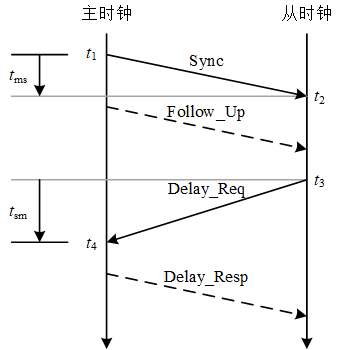
\includegraphics[width=0.5\textwidth]  {fig10.png}} 
	\caption{同步过程中的时间戳交互}
\end{figure}

\subsection{本章小节}
本章主要探讨了5G+TSN异构网络的混合时钟同步方法。首先针对核心网内部的5G+TSN网络部分,进行了子载波间隔优化以解决同步精度和带宽利用率之间的trade-off问题,同时为了减小误码率,引入了均衡器来改善系统性能,设计了适合5G网络的自适应判决反馈均衡器(Adaptive DFE)。ADFE能够实现高性能、自适应和复杂度可控的优点,适应5G网络的高速度、大带宽和动态复杂信道环境的特点。

最后,本章还阐述了针对大规模5G-TSN的时间戳补偿算法。当多个网桥相互连接时,需要对时间戳进行补偿和校正,以提高同步精度。
\newpage
\fancyhead[LH]{上海交通大学学位论文}
\fancyhead[RH]{第四章\quad仿真实验}
\section{仿真实验}
\subsection{分层算法仿真}

首先需要对第二章提出的混合架构分层算法进行仿真,先通过一个简答的实例来说明原理,再进行大规模复杂网络的仿真实验。
\begin{figure}[htb] 
	\center{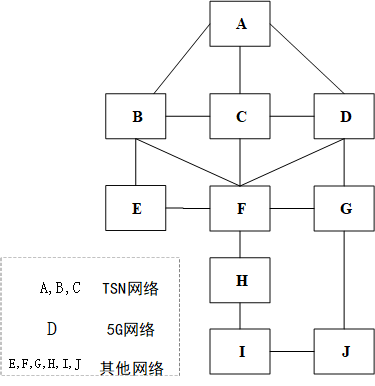
\includegraphics[width=0.95\textwidth]  {fig31.png}} 
	\caption{分层前的网络拓扑}
\end{figure}
\begin{figure}[htb] 
	\center{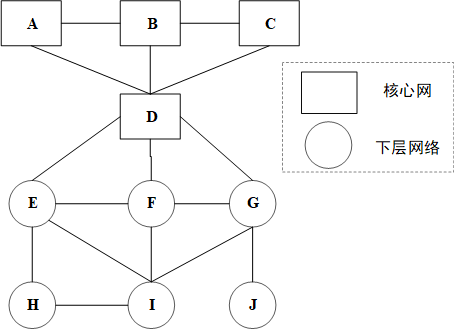
\includegraphics[width=0.95\textwidth]  {fig32.png}} 
	\caption{分层后的网络拓扑}
\end{figure}
在这个实例中,我们为每个参数赋予具体的数值。例如,我们可以假设以下参数值:

\begin{itemize}
	\item 时钟偏差($\Delta T$)和频率偏差($\Delta f$):
	\begin{enumerate}
		\item 节点A: $\Delta T_A = 1 \text{ns}, \Delta f_A = 0.1 \text{ppm}$
		\item 节点B: $\Delta T_B = 2 \text{ns}, \Delta f_B = 0.2 \text{ppm}$
		\item 节点C: $\Delta T_C = 3 \text{ns}, \Delta f_C = 0.15 \text{ppm}$
	\end{enumerate}
	
	\item 确定性延迟($L_{ij}^D$)和随机延迟($L_{ij}^R$):
	\begin{enumerate}
		\item 连接AB: $L_{AB}^D = 10 \text{ns}, L_{AB}^R = 2 \text{ns}$
		\item 连接AC: $L_{AC}^D = 15 \text{ns}, L_{AC}^R = 3 \text{ns}$
		\item 连接BC: $L_{BC}^D = 12 \text{ns}, L_{BC}^R = 2.5 \text{ns}$
		\item 连接AD: $L_{AD}^D = 20 \text{ns}, L_{AD}^R = 4 \text{ns}$
	\end{enumerate}
	
	\item 到达率($\lambda_D$)和排队等待时间($W_D$):
	\begin{enumerate}
		\item 节点D: $\lambda_D = 100 \text{packets/s}, W_D = 1 \text{ms}$
	\end{enumerate}
	
	\item 同步误差($E_{ij}$):
	\begin{enumerate}
		\item 节点A和E之间:$E_{AE} = 5 \text{ns}$
		\item 节点A和F之间:$E_{AF} = 7 \text{ns}$
		\item 节点B和G之间:$E_{BG} = 6 \text{ns}$
	\end{enumerate}
	
	\item NSPI的权重:
	\begin{enumerate}
		\item $W1 = 0.4$
		\item $W2 = 0.3$
		\item $W3 = 0.3$
	\end{enumerate}
\end{itemize}

根据这些参数值,我们可以计算出每个节点的NSPI值,并进行分层,对于大规模网络,分层的本质就是一种聚类算法,具体的步骤如下:
构建时钟模型:为顶层TSN节点A、B、C,5G节点D,以及其他网络节点E、F、G、H、I、J构建综合时钟模型。对于每个节点,我们需要考虑其时钟偏差($\Delta T$)和频率偏差($\Delta f$)。例如,节点A的时钟模型可以表示为$T_A(t) = t + \Delta T_A + \Delta f_A \cdot t$。

延迟建模与分析:为每对相邻节点之间的连接分析确定性延迟和随机延迟。例如,为连接AB、AC、BC、AD、BD、CD、DE、DF、DG等建立延迟模型。我们可以使用公式$L_{ij} = L_{ij}^D + L_{ij}^R$表示节点i和j之间的总延迟,其中$L_{ij}^D$表示确定性延迟,$L_{ij}^R$表示随机延迟。

排队延迟计算:对于5G节点D,我们可以使用Little公式计算其与其他节点(如E、F、G)同步时产生的排队延迟。设$N_D$为节点D的排队长度,$\lambda_D$为到达率,$W_D$为排队等待时间,则有$N_D = \lambda_D \cdot W_D$。

评估累积同步误差:在这个拓扑中,我们需要分析从顶层TSN节点A、B、C到底层节点I、J的累积同步误差。设$E_{ij}$为节点i和j之间的同步误差,则累积同步误差可表示为$E_{total} = \sum_{i,j} E_{ij}$。

混合同步架构的建立与优化:根据网络同步性能指标(NSPI)的计算结果,我们可以确定每个节点所属的层级。使用公式$NSPI = (W1 * SPW * \delta) + (W2 * (1 - SPW) * (n * \beta * (1 + p) / \mu)) + (W3 * D_{\text{RMSE}})$计算每个节点的NSPI值。分层后的拓扑结构如图4-7所示。

再完成简单实例后,将会对大规模复制网络节点进行分层仿真,为了说明大规模网络中的分层算法效果,我们针对以下参数进行仿真设置
\begin{enumerate}
	\item 节点数量:$N = 10000$
	\item 空间范围:$X = [0, 100], Y = [0, 100], Z = [0, 100]$
	\item 层级数量:$L = 4$
	\item 分层算法:分层算法采用的是我们前面提到的基于聚类的方法,即对$(x, y, z)$坐标进行聚类分析,将节点划分到不同的层次。
	\item 路径选择概率:在分层前,每个节点从所有其他节点中随机选择一个节点进行通信,因此路径选择概率为$\frac{1}{N-1}$。分层后,节点只与同一层内的其他节点通信,假设每层的节点数量为$N_i$,则路径选择概率为$\frac{1}{N_i-1}$。
	\item 网络冲突参数:在分层前,我们可以计算整个网络的平均路径选择概率为$P_{\text{avg}} = \frac{1}{N-1}$。因此,任意两个节点之间的通信路径重合的概率为$P_{\text{overlap}} = P_{\text{avg}}^2$。分层后,不同层之间的通信路径不会重合,因此可以降低网络冲突。
	\item 时延参数:在分层前,我们可以假设所有节点之间的通信时延为均匀分布的随机变量,其范围为$[T_{\text{min}}, T_{\text{max}}]$。分层后,由于节点之间的通信距离减小,我们可以假设通信时延的范围缩小为$[T_{\text{min}}', T_{\text{max}}']$,其中$T_{\text{min}}' \ge T_{\text{min}}, T_{\text{max}}' \le T_{\text{max}}$。
\end{enumerate}
\begin{figure}[H] 
	\center{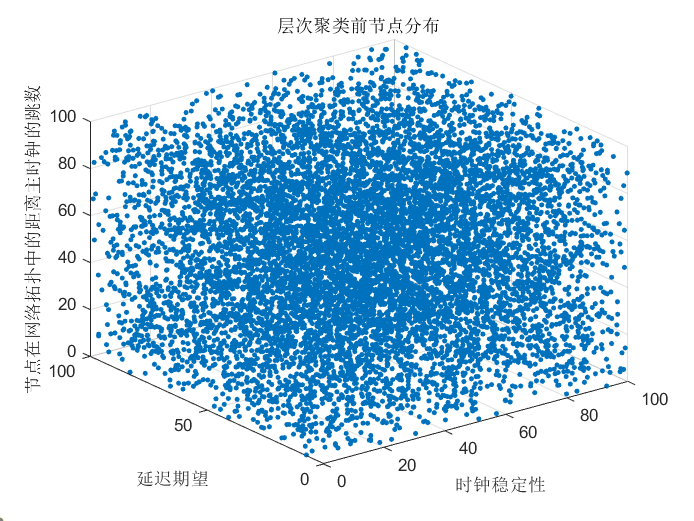
\includegraphics[width=0.95\textwidth]  {fig33.png}} 
	\caption{大规模网络分层前}
\end{figure}

图4.3展示了分层前的节点分布示意图。在这个图中,x轴、y轴和z轴分别代表了节点的三个关键属性:时钟稳定性(Clock Stability, CS)、延迟期望(Latency Expectation, LE)以及节点在网络拓扑中的位置(Synchronization Hierarchy Level, SHL)。时钟稳定性和延迟期望是衡量节点时钟性能的两个重要指标,它们对于同步系统的准确性和稳定性至关重要。

为了对节点进行评估并进行适当的分层,首先需要计算每个节点的节点同步性能指数(Node Synchronization Performance Index, NSPI)。NSPI是一个综合指标,它综合考虑了时钟稳定性和延迟期望,以便对节点的同步性能进行量化评估。通过计算每个节点的NSPI值,可以在同步系统中对节点进行排序,从而确定节点在分层拓扑中的相对位置。

在确定了节点的NSPI值后,接下来需要采用一种分层聚类算法来对节点进行分层。分层聚类算法的目标是将具有相似性能(即具有相近NSPI值)的节点聚集到同一层级上。在执行此过程时,算法应尽量保证累计误差最小化,以确保同步系统的准确性和稳定性。

综上所述,图4.3为我们提供了一个关于节点分布的直观表示,通过对节点时钟稳定性、延迟期望以及在拓扑中的位置进行量化分析,我们可以使用NSPI值和分层聚类算法来对节点进行分层,从而实现同步系统的优化。在优化过程中,需要充分考虑最小化累计误差的约束,以确保整个同步系统具有高度的准确性和稳定性。。
\begin{figure}[H] 
	\center{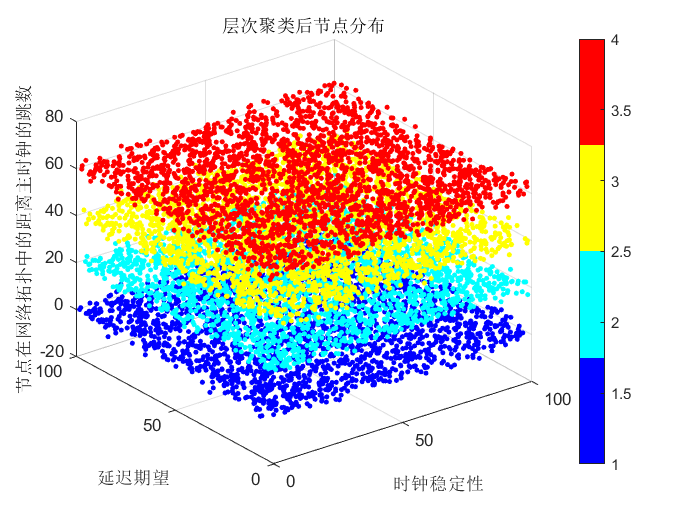
\includegraphics[width=0.95\textwidth]  {fig34.png}} 
	\caption{大规模网络分层后}
\end{figure}

图4.4为分层后的节点分布示意图,通过分层聚类的算法,可以将时钟性能相近的节点分在同一层。可以看到聚类算法非常有效地将节点分成了四层,在图4-9中,不同颜色代表了不同的层级,右侧颜色轴上的数字代表了NSPI值。

完成分层后,节点将遵循第二章中的初始化同步算法进行同步,通过仿真可以得到分层前后同步效果的对比图4.5。
\begin{figure}[H] 
	\center{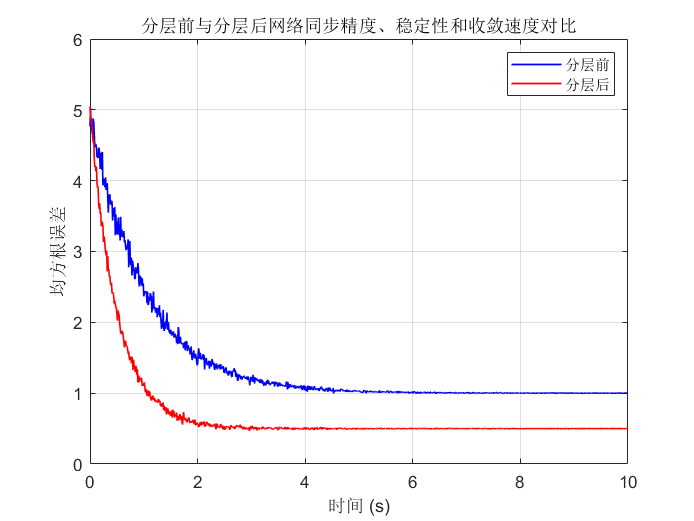
\includegraphics[width=0.95\textwidth]  {fig35.png}} 
	\caption{分层前后同步性能对比}
\end{figure}

对比的性能为第二章中提到的收敛速度和时钟稳定性,横轴为同步时间,纵轴为均方根误差,为了方便观察,将初始同步精度误差设置为较小的$5\mu s$,可以看到分层后时钟误差收敛速度明显快于分层前。分层前收敛时间为5.03s,分层后收敛时间为3.14s,且分层前最后收敛于$1\mu s$左右,分层后最后收敛于490ns左右。可以得出结论,通过混合架构的分层算法,有效提高了时钟同步的性能。
\subsection{核心网络5G+TSN时钟同步优化仿真}
\subsubsection{载波间隔优化仿真}
基于第2章和第3章提出的同步体系结构和模型,我们进行了数值模拟来评估优化和补偿方案的性能。我们首先检查了不同子载波间隔(SCS)值下的同步精度。根据5G NR系统的数学规范设置\textsuperscript{\cite{access2015requirements}},最大的SCS为480 kHz,傅里叶变换(FFT)大小为4096,导致时间单位为0.509 ns。我们假设5G内部UE时钟相对于gNB时钟的漂移率$\frac{\alpha_{5G}}{\alpha_{TSN}}$为10 ppm(每毫秒10 ns)。表4.1显示了模拟结果。

\begin{table}[!htb]
	\centering
	\caption{不同载波间隔对应的同步误差}
	\label{tab1}
	\begin{tabular}{l|l|l}
		\hline
		& \textbf{平均误差(ns)}& \textbf{最大误差(ns)} \\
		\hline
		15kHz 
		& 896
		& 2525 \\
		\hline
		30kHz
		& 425
		& 1295 \\
		\hline
		60kHz
		& 295
		& 899 \\
		\hline
		120kHz
		& 135
		& 578 \\
		\hline
		240kHz
		& 120
		& 512 \\
		\hline
		480kHz
		& 112
		& 508 \\
		\hline
	\end{tabular}
\end{table}


我们观察到,随着SCS的增加,同步误差减小。然而,当SCS达到120 kHz时,误差减小速度变慢,当它达到240 kHz时,误差大小趋向于一个恒定值。随后,同步精度和带宽利用权重($\omega_1,\omega_2$)分别被设置为(0.5,0.5)。通过解决第4节中提出的优化问题,当载波带宽为120 kHz时,获得了最佳性能。此时,总可用带宽长度为393.12 MHz,实现了5G网络的最高利用率98\%,可用带宽利用率为83.38\%,满足了大多数传输要求。
\subsubsection{均衡器仿真}
在载波间隔确定后,为降低误码率的影响,我们需要进行均衡器补偿仿真。该仿真主要针对基带信号,不涉及射频内容。接收端输入信号rxWaveform已经为IQ路数据,SSB只能处在同步栅格上。同步栅格是用于配置同步/广播信号的基本频率位置,是一个绝对频率。可以将rxWaveform理解为接收端已经从同步栅格频率下变频到基带,并完成A/D采样后所得到的基带数据。对这些基带数据通过一系列算法来判断数据中是否包含SSB同步块。如果存在,则说明已经找到同步块并成功恢复MIB。

为了实现这一目标,我们采用了“时频二维搜索”方法,并通过遍历NID2的三种情况来完成粗频偏估计和确定NID2。搜索间隔(或搜索步长)决定了第一层for循环应以多大的频率间隔进行搜索。这也对应于代码中的fshifts设置。搜索间隔实际上是频率分辨率,比搜索间隔还小的频率偏差,接收机此时无法分辨出具体的频率偏差值。在MATLAB 5G工具箱中,搜索步长的设置为1/2*scs。这是因为基于CP的CFO估计技术能估计的范围是子载波间隔乘以[-0.5,0.5),该技术不能用于估计整数倍频偏。所以在采用基于CP的CFO估计技术之前,需要将频率间隔误差估计到子载波间隔乘以[-0.5,0.5)之内。

在信道均衡方面,我们先采用了MMSE均衡器,即考虑了噪声的ZF均衡器。信道估计和均衡的目的是不同的:信道估计的目的是通过收发双方都已知的一段导频序列(例如发送端发送导频序列x=[1,1,1,1,1],经过信道后到达接收端,假设为y),因为收发两端均知道x,接收端又有收到的y,便估计出H。信道估计就是已知y和x,求H。信号均衡的目的则是接收端通过已经接收到的y,和之前已经通过信道估计得到的H,来补偿信道对于信号的影响,从而更有效地恢复出x。

为了实现自适应判决均衡器的仿真设计,我们在原有基础上引入自适应算法,以便在动态变化的信道环境中实现更优的性能。自适应判决均衡器的主要目标是通过在线更新均衡器系数,以便在不同信道条件下更好地追踪信道特性。在实现过程中,我们可以采用最小均方误差(LMS)算法或其变种,如归一化最小均方误差(NLMS)算法、递推最小二乘法(RLS)等。

在仿真中,我们首先将输入的基带数据传输到自适应判决均衡器,然后根据当前的信道状态和均衡器系数,计算误差信号。接下来,我们通过更新均衡器系数以最小化误差信号,从而实现自适应调整。在整个过程中,我们需要监控均衡器的性能,例如跟踪误差和收敛速度,并与其他类型的均衡器进行比较,以验证自适应判决均衡器的有效性。
首先,我们初始化自适应判决均衡器的参数,包括滤波器长度($L$),步长因子($\mu$),以及权重向量($\boldsymbol{w}$)。滤波器长度决定了均衡器的时域响应范围,通常需要根据信道特性和信号类型进行选择。步长因子影响了均衡器的收敛速度和稳定性,较大的步长因子可以加快收敛速度,但可能导致稳定性降低。权重向量用于存储当前的均衡器系数。
在每个时刻$t$,我们接收到基带数据($\textit{rxWaveform}$)的一个样本($r_t$),并将其与当前的权重向量($\boldsymbol{w}$)进行卷积,得到判决输出($y_t$)。然后,我们计算期望信号($d_t$)与判决输出($y_t$)之间的误差信号($e_t = d_t - y_t$),并用于更新权重向量($\boldsymbol{w}$)。权重向量的更新公式如下:
\begin{equation}
	\boldsymbol{w}_{t+1} = \boldsymbol{w}_t + \mu \cdot e_t \cdot \frac{\boldsymbol{r}_t}{\Vert \boldsymbol{r}_t \Vert^2 + \epsilon}
\end{equation}
其中,$\epsilon$ 是一个很小的正数,用于防止除零错误。在整个更新过程中,我们需要注意权重向量的收敛速度和稳定性,并调整步长因子($\mu$)以实现较好的性能。

为了评估自适应判决均衡器的性能,我们可以采用误码率(BER)或信噪比(SNR)等指标。在仿真过程中,我们可以通过比较自适应判决均衡器与其他类型均衡器(如MMSE均衡器)的性能,进一步验证其优越性。此外,我们还可以研究不同参数设置下自适应判决均衡器的性能变化,以找到最佳参数组合。

采总之,自适应判决均衡器通过在线更新均衡器系数,能够在动态变化的信道环境中实现更优的性能。具体到参数仿真,我们可以采用归一化最小均方误差(NLMS)算法来实现自适应判决均衡器,并通过评估误码率(BER)或信噪比(SNR)等指标来验证其性能。在实际应用中,我们需要根据信道特性和信号类型选择合适的滤波器长度,并调整步长因子以实现较好的收敛速度和稳定性。
\begin{figure}[htb] 
	\center{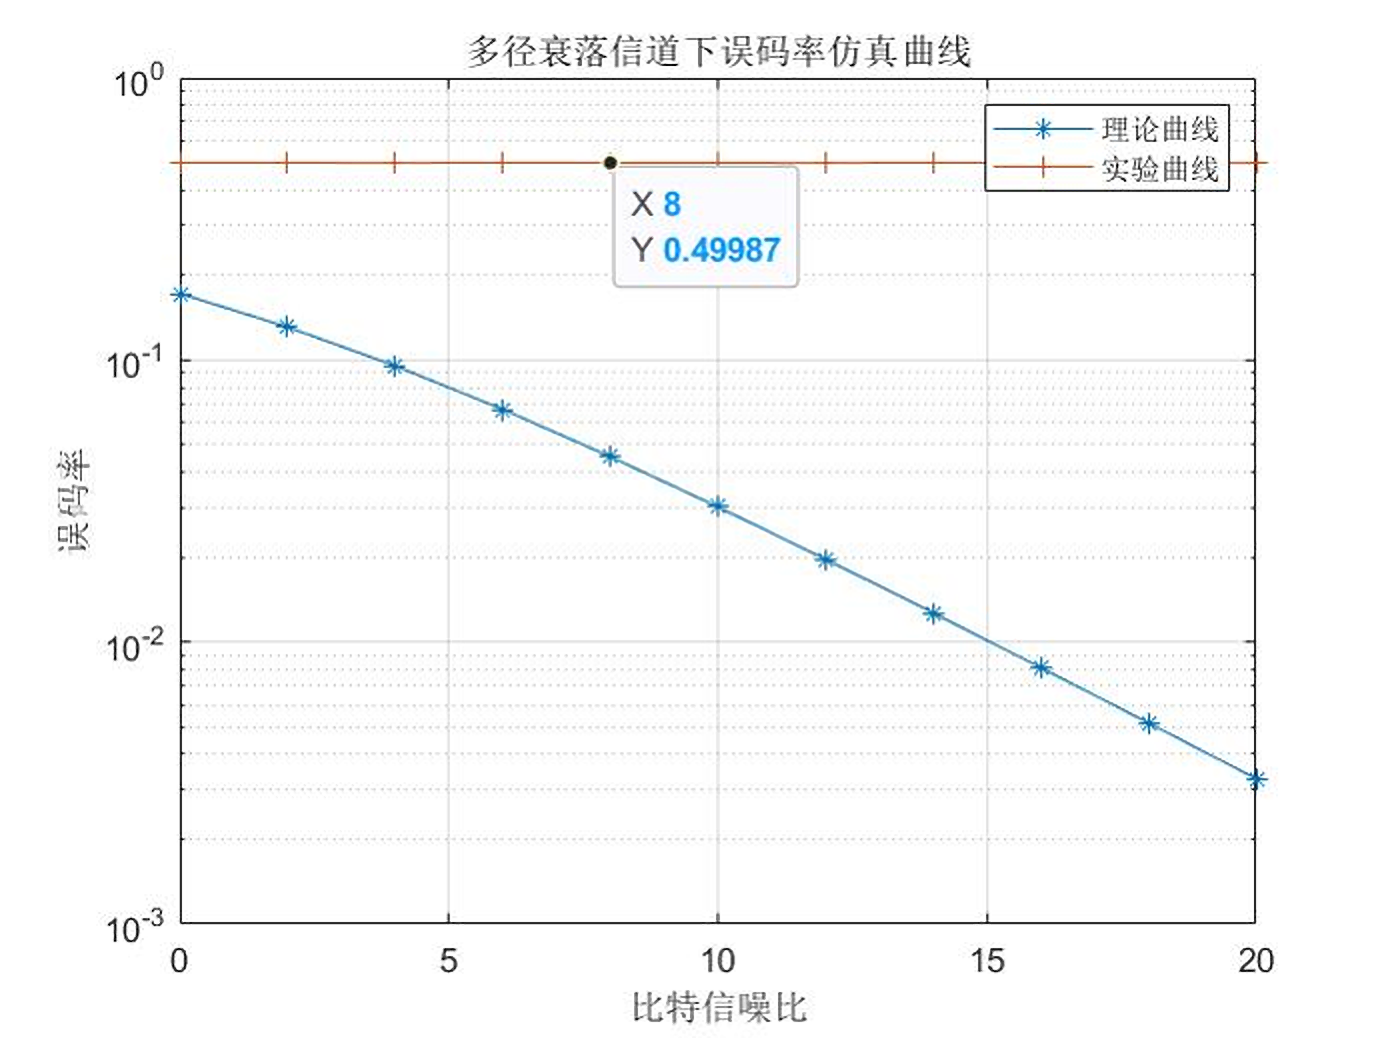
\includegraphics[width=0.95\textwidth]  {fig38.png}} 
	\caption{添加均衡器之前的误码率曲线}
\end{figure}
\begin{figure}[htb] 
	\center{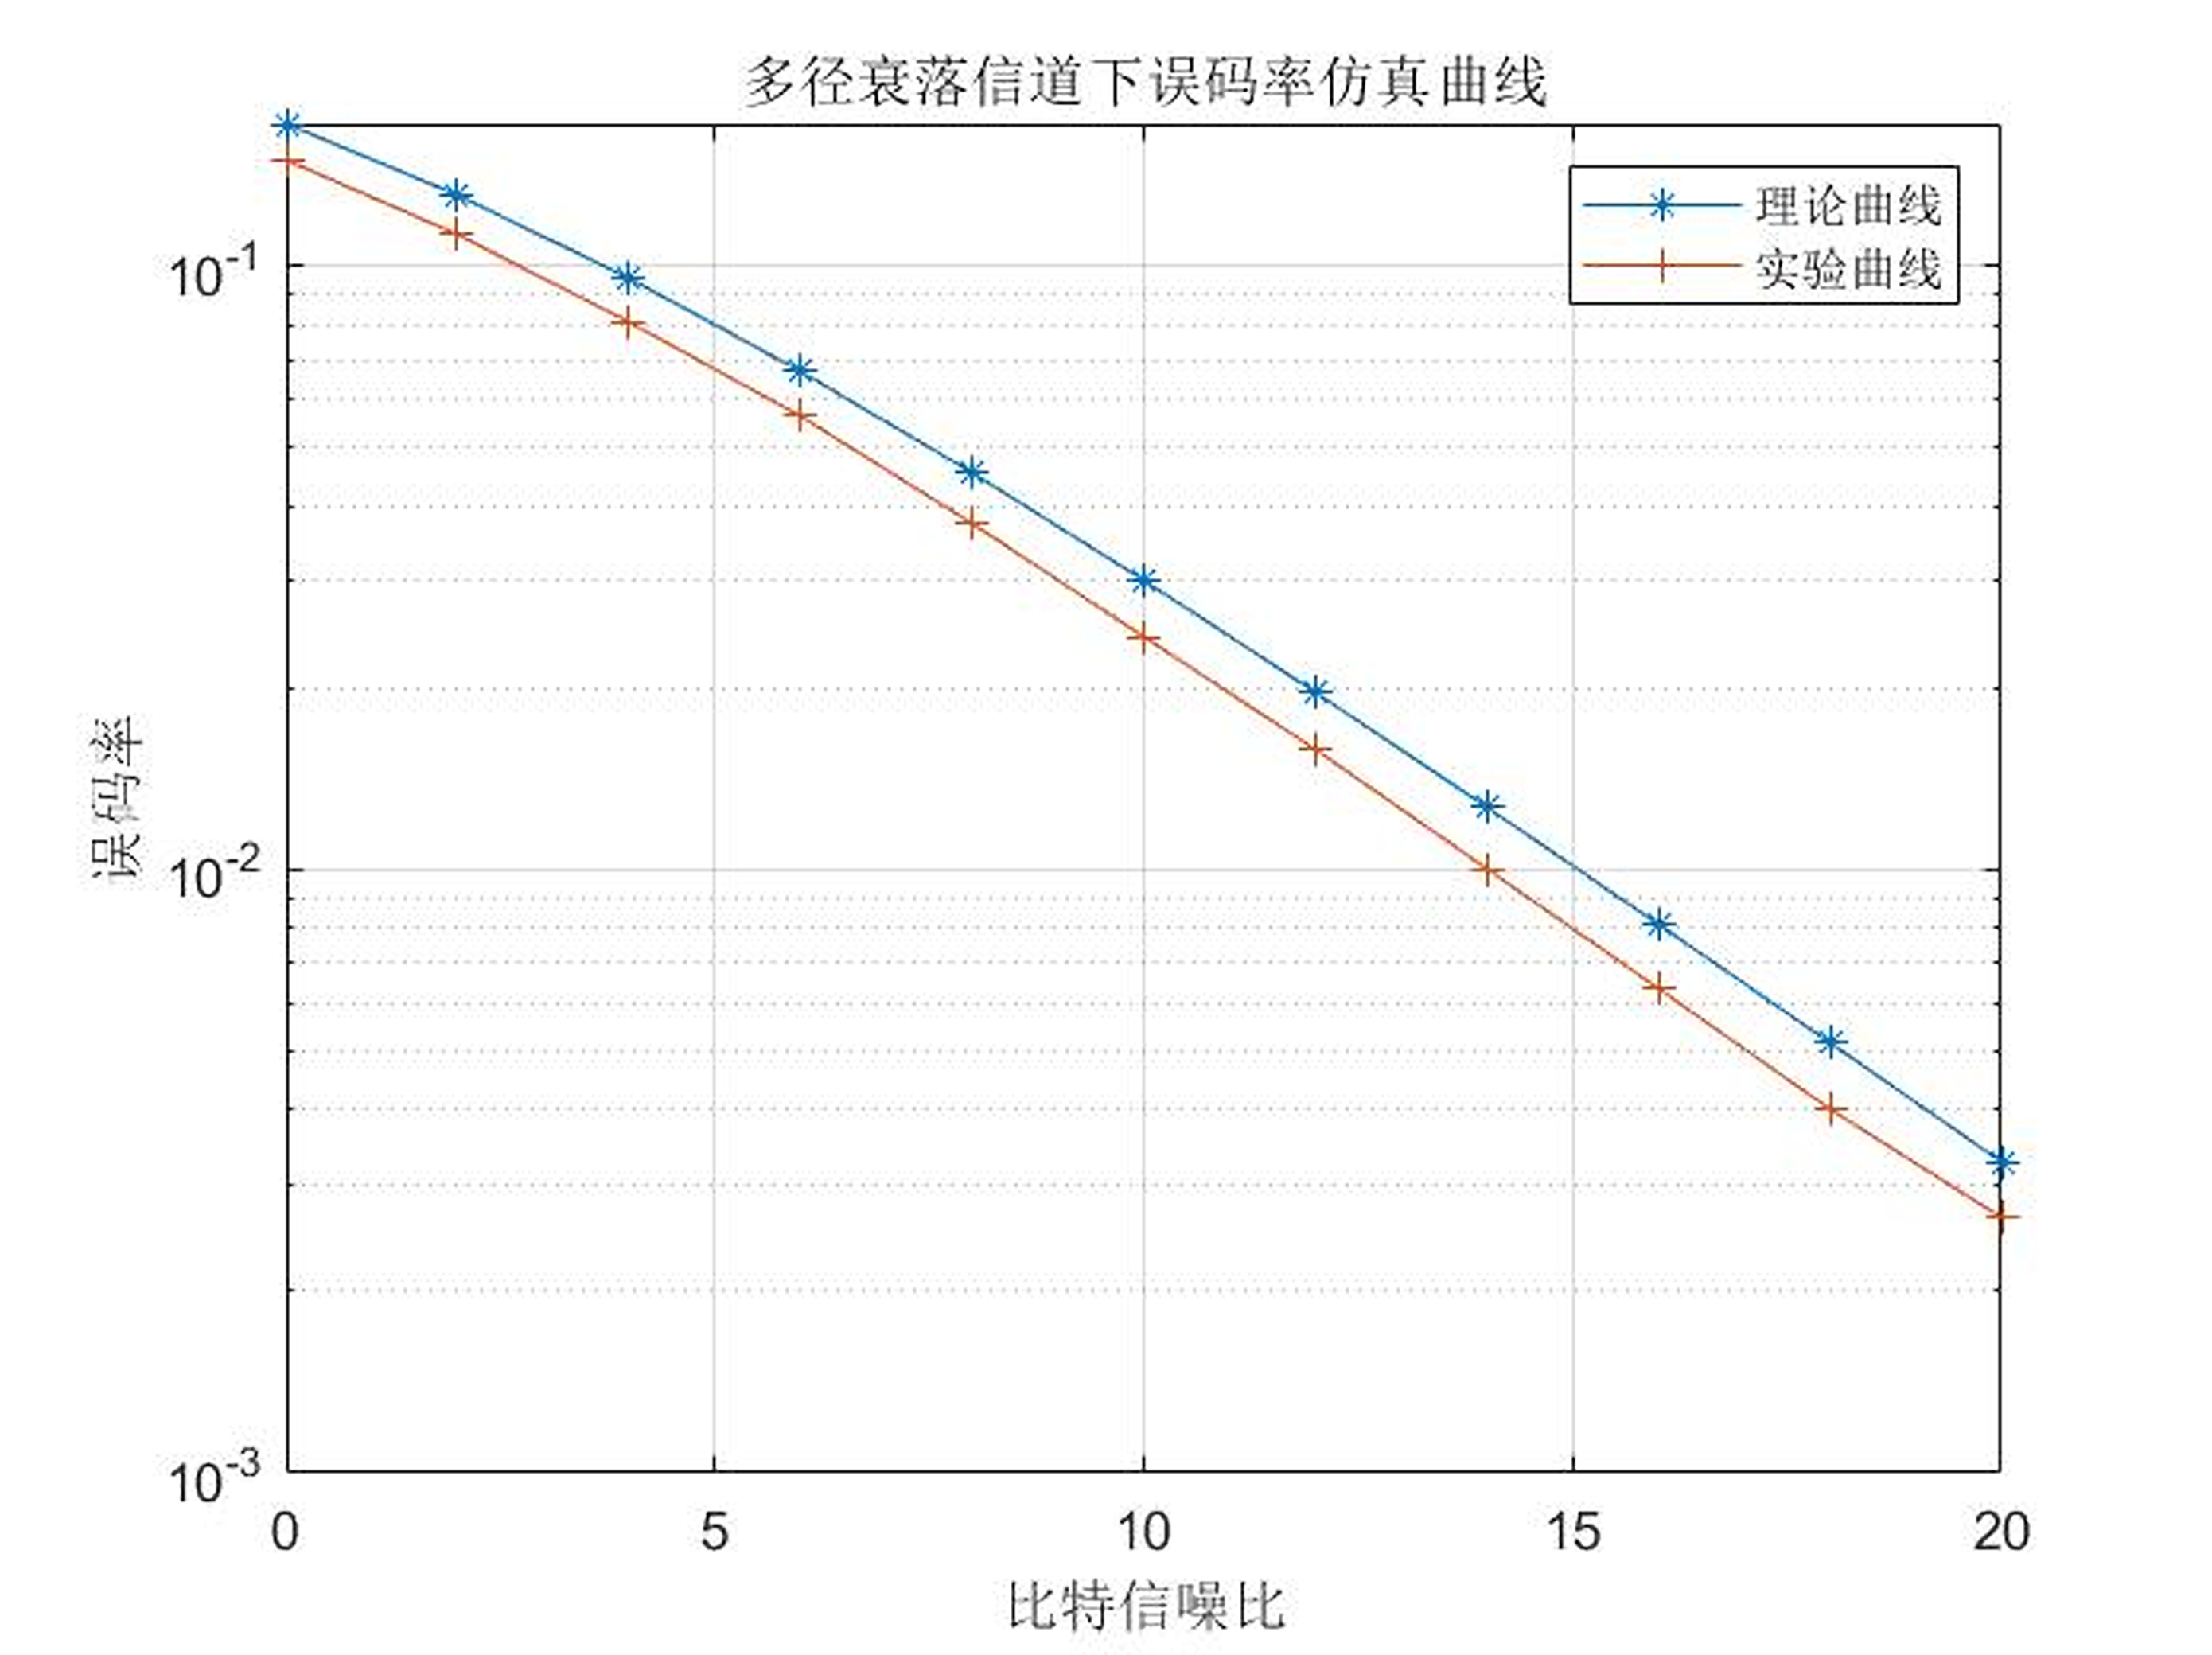
\includegraphics[width=0.95\textwidth]  {fig39.png}} 
	\caption{添加均衡器之后的误码率曲线}
\end{figure}
图4.6和图4.7分别表示了在添加MMSE均衡器前后的误码率与信噪比的关系。可以看到在在进行均衡器补偿之前,误码率并没有随着信噪比增加而降低,这就是多晶衰弱造成的影响。但该实验仅针对理想情况,下面将展示在更复杂信道情况下的MMSE与自适应判决反馈均衡器的对比。
\paragraph{MMSE与ADFE的对比实验}
这次仿真实验目的是比较两种均衡器策略:最小均方误差(MMSE)均衡器和自适应判决反馈(ADFE)均衡器在不同信噪比(SNR)条件下的误码率(BER)在大规模复杂网络环境下的性能。首先生成N=10000个二进制符号的随机数据,然后通过二进制相移键控(BPSK)调制得到调制信号。接下来,通过一个具有三个路径和10dB瑞利系数的瑞利信道模型发送调制信号。

对于每个信噪比,分别对信道输出信号添加高斯白噪声,然后分别用MMSE均衡器和ADFE均衡器处理接收信号。MMSE均衡器通过计算信道冲激响应的频域倒数来最小化均方误差。而ADFE均衡器则采用归一化最小均方误差算法,使用步长因子mu = 0.01和长度L = 5来自适应地调整权重。

接收信号经过两种均衡器处理后,对信号进行BPSK解调,然后计算与原始数据的误码率。最后,将MMSE和ADFE均衡器在不同信噪比下的误码率绘制在一张图上。
\begin{enumerate}
	\item \textbf{参数设置}
	\begin{itemize}
		\item 符号数(N):我们选择了10000个符号进行仿真。
		\item 均衡器长度(L):均衡器的长度被设置为5。
		\item 步长因子(mu):对于ADFE算法,步长因子被设置为0.01。
		\item 信噪比向量(snrVec):我们选择了从0dB到30dB,步长为2dB的信噪比范围进行仿真。
	\end{itemize}
	
	\item \textbf{随机数据生成}
	\begin{itemize}
		\item 生成10000个随机比特符号。
		\item 使用二进制相移键控(BPSK)调制将比特符号映射到符号。
	\end{itemize}
	
	\item \textbf{信道定义}
	\begin{itemize}
		\item 定义了一个瑞利信道,路径功率分布为[0.9 0.3 0.1],归一化后的路径功率分布为[0.643 0.214 0.071]。
		\item 设置瑞利信道的K因子为10,表示信道中存在直射信号成分。
		\item 信道中的多径延迟设置为[0 1 2]。
	\end{itemize}
	
	\item \textbf{误码率性能仿真}
	\begin{itemize}
		\item 对于每个信噪比值,执行以下步骤:
		\begin{enumerate}
			\item 通过瑞利信道发送调制信号。
			\item 向信道输出添加高斯白噪声,以达到指定的信噪比。
			\item 使用MMSE均衡器处理接收信号。
			\item 使用自适应判决反馈均衡器(NLMS算法)处理接收信号。
			\item 计算MMSE均衡器和自适应判决反馈均衡器的误码率。
		\end{enumerate}
	\end{itemize}
	
	\item \textbf{结果绘图}
	\begin{itemize}
		\item 绘制误码率随信噪比变化的曲线,比较MMSE均衡器和自适应判决反馈均衡器的性能。
	\end{itemize}
	
	\item \textbf{在设计过程中遇到的问题}
	\begin{itemize}
		\item 选择合适的信道模型:最初使用了错误的信道模型。我们纠正了问题,选择了瑞利信道模型。
		\item 正确配置信道参数:在配置瑞利信道参数时,我们遇到了一些错误,例如设置无效属性,K因子设置为零等。我们逐一解决了这些问题,正确地配置了信道参数。
		\item 选择正确的均衡器算法:最初,我们错误地将MMSE均衡器的算法属性设置为"MMSE",而正确的属性值应该是"LMS"、"RLS"或"CMA"。为了解决这个问题,我们改用\texttt{comm.LinearEqualizer}类,并将算法属性设置为"LMS",同时将参考系数调整为1,以实现MMSE均衡器。
		\item 处理不匹配的输入和输出尺寸:在处理信号时,需要确保输入和输出尺寸正确匹配。我们遇到了一些不匹配的输入和输出尺寸问题,通过调整输出尺寸以匹配原始数据大小来解决这些问题。
	\end{itemize}
\end{enumerate}

仿真结果如图4.8所示,可以看到在大规模复杂网络的应用场景下,由于信道的干扰较多,MMSE均衡器未能很好的降低误码率,其误码率水平一直维持为0.4802左右,而自适应判决反馈均衡器则成功将误码率控制0.0305附近。可以得知当载波间隔较高时,通过自适应反馈均衡器,可以有效地降低大规模复杂异构网络的误码率,从而使得载波优化不会影响到普通传输。
\begin{figure}[H] 
	\center{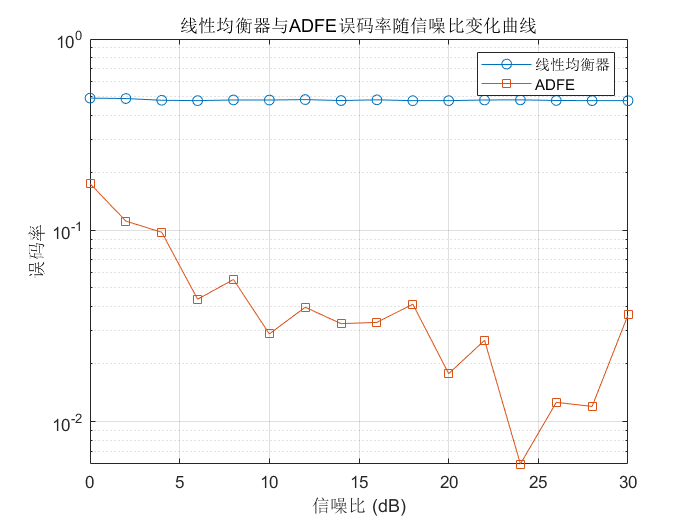
\includegraphics[width=0.95\textwidth]  {fig37.png}} 
	\caption{MMSE均衡器与自适应判决反馈均衡器对比}
\end{figure}
\subsubsection{时间戳补偿仿真}。
我们在确定最适合的载波间隔后进行了时间戳补偿的仿真。我们将工业现场的无线节点建模为连接到5G UE的TSN终端,通过可变数量的网桥(在本例中为透明时钟)连接到其上。TSN和5G设备都基于omnet节点类型。节点类型的建立如下所述:
\begin{itemize}
	\item 网络中的TSN节点也是通过载波感应多路存取(CSMA)信道模型连接的,它支持第二层通信,并满足802.1AS的规范要求。一个单独的类定义了安装在每个节点上的gPTP程序。节点类型分为边界时钟和公共时钟,这决定了它们不同的行为模式。普通节点从主时钟接收同步信息并执行传输延迟测量程序,而边界节点在收到5G节点的同步要求后作为主时钟执行传输延迟测量程序。
	\item 在5G网络中,5G-TSN网桥是最关键的组成部分。在OMNeT++仿真中,网桥的协议转换器由两个节点类定义:一个作为有线端口,负责连接到CSMA信道,而另一个被设置为5G模块,作为无线端口,连接到无线信道。两个节点共享一个本地时钟实例,反映了它们位于同一设备内的事实。网桥内的5G节点使用5G LENA模块进行通信,该模块专注于PHY和MAC层,实现无线信道,并支持各种帧结构和频段。
\end{itemize}
网络节点以二叉树结构组织。多个桥的错误有一个相互抵消的概率,导致错误大小在一定范围内波动。为了研究它,我们对网络中每个不同数量的桥进行了100次模拟,结果如图7所示。
\begin{figure}[htb] 
	\center{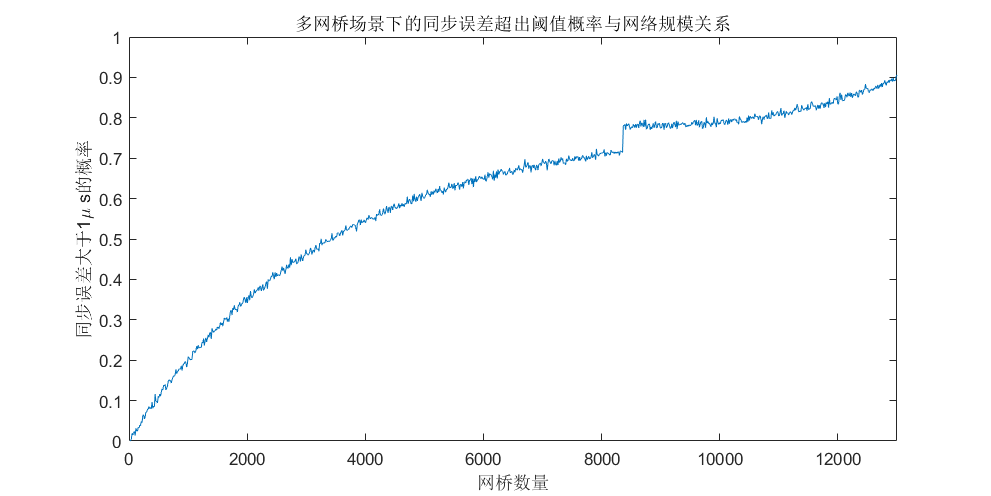
\includegraphics[width=0.95\textwidth]  {fig25.png}} 
	\caption{多网桥场景下的同步误差越界概率与网络规模关系}
\end{figure}

图4.8显示了同步误差大于1$\mu s$的概率与网络规模之间的关系,网络规模由网络中的5G-TSN网桥数量表示。随着网络规模和网桥数量的增加,同步误差超过最低精度要求的概率也在增加。当网桥数量达到13000个时,同步误差超过1$\mu s$的概率在90\%以上。因此,我们应用算法进行时间戳补偿,补偿前后的结果比较如下:
\begin{figure}[htb] 
	\center{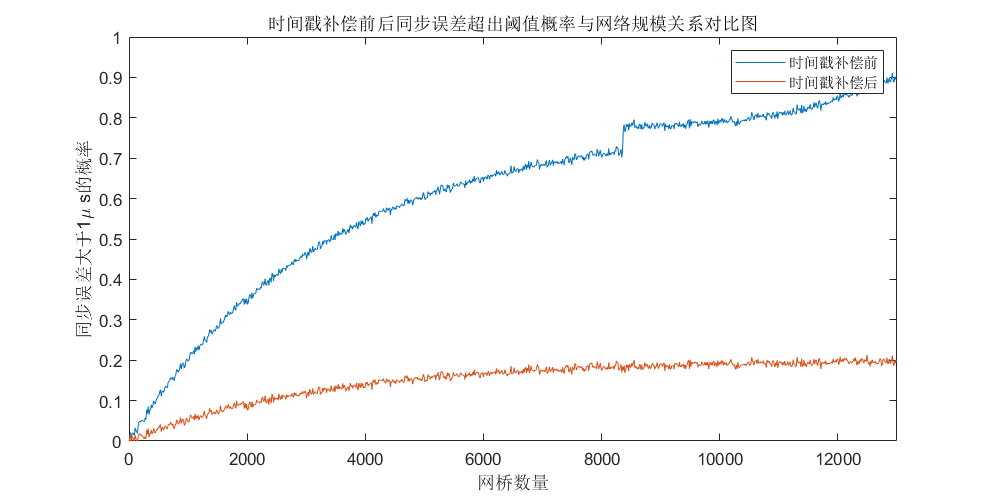
\includegraphics[width=0.95\textwidth]  {fig24.png}} 
	\caption{多网桥场景下的同步误差越界概率与网络规模关系}
\end{figure}

图4.9说明,补偿后同步误差超过1$\mu s$的概率大大降低,保持在20\%以内。图4.10显示了补偿前后平均同步误差的变化。可以看出,当网络规模达到10,000或更大时,补偿前的平均同步误差达到约10微秒。然而,经过补偿后,平均同步误差被控制在900ns以内,有效地提高了使用集成5G和TSN的系统的同步精度。
\begin{figure}[H] 
	\center{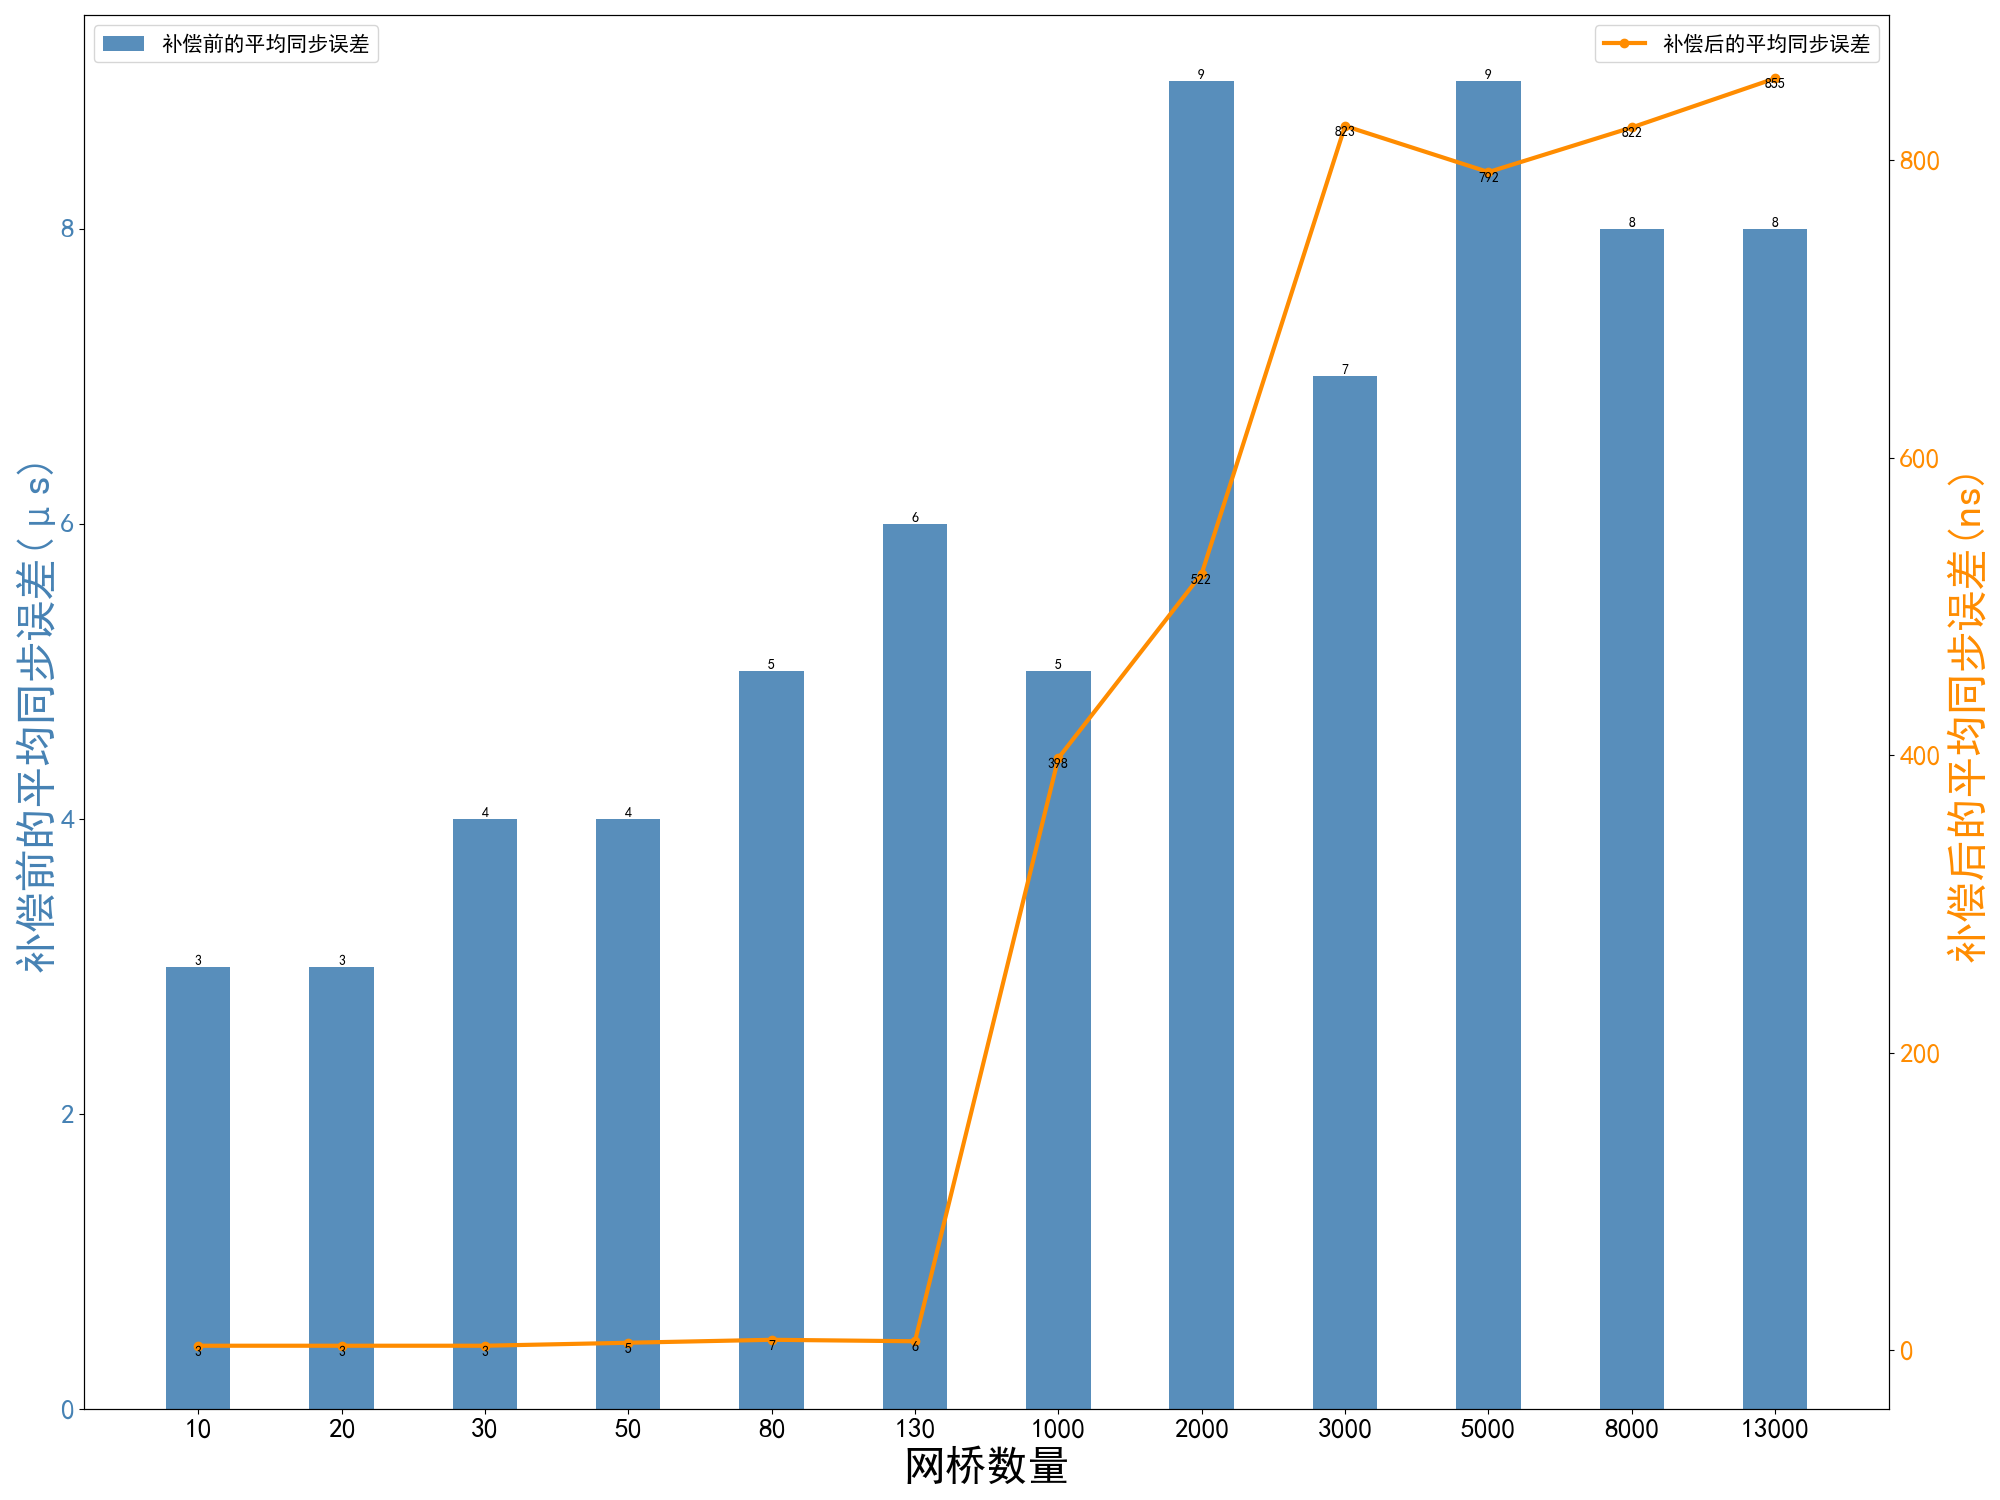
\includegraphics[width=0.95\textwidth]  {fig23.png}} 
	\caption{时间戳补偿前后平均同步误差与网络规模关系对比}
\end{figure}


\subsection{本章小结}
本章通过仿真实验验证了混合架构分层算法在时钟同步性能上的优势。首先通过一个简单实例阐述分层算法原理,接着进行大规模复杂网络的仿真实验。实验结果显示分层后时钟误差收敛速度明显快于分层前,且同步精度更高。

此外,本章还介绍了5G+TSN时钟同步优化仿真,分析了不同子载波间隔(SCS)值下的同步精度。结果表明随着SCS增加,同步误差减小,通过构建优化问题,找到了在同步精度和带宽利用率之间取得平衡的载波间隔。同时,为降低误码率,进行了均衡器仿真,比较了ADFE与MMSE在在大规模复杂网络环境下的性能,仿真结果显示,自适应判决反馈均衡器在应对信道干扰方面表现优越,将误码率成功控制在0.0305附近,而MMSE均衡器的误码率保持在0.4802左右。因此,在大规模复杂异构网络中,自适应判决反馈均衡器更能有效降低误码率,使得载波优化不会影响普通传输。另外,本节还介绍了时间戳补偿仿真,通过建立工业现场的无线节点模型,并以二叉树结构组织网络节点,评估了多网桥场景下的同步误差越界概率与网络规模关系。补偿后的结果显示,同步误差大幅降低,平均同步误差在900ns以内,有效提高了集成5G和TSN系统的同步精度。

总之,本章通过对混合架构分层算法、载波分配算法、自适应判决反馈均衡器补偿和时间戳补偿的仿真实验,验证了这些算法设计在大规模复杂网络场景下的效果。


\newpage
\fancyhead[LH]{上海交通大学学位论文}
\fancyhead[RH]{第五章\quad全文总结}
\section{全文总结}

\subsection{工作总结}
本课题研究了时钟同步在有线和无线异构网络中的应用,针对现有研究在大规模复杂异构网络中的适用性、动态性和可扩展性、安全性和鲁棒性等方面存在的缺陷,提出了一种基于5G-TSN核心网络的混合架构时钟同步解决方案。主要工作总结如下:

设计了一种有线/无线网络混合时钟同步架构,引入了名为“网络同步性能指标(NSPI)”的综合评估指标,用于网络分层。采用预处理方法对有向图进行处理,实现井然有序的时钟同步,并提高同步效率,降低同步延迟和抖动。

通过仿真实验验证了混合架构分层算法在时钟同步性能上的优势。实验结果显示分层后时钟误差收敛速度明显快于分层前,且同步精度更高。同时,进行了5G+TSN时钟同步优化仿真,分析了不同子载波间隔(SCS)值下的同步精度。通过构建优化问题,找到了在同步精度和带宽利用率之间取得平衡的载波间隔。

对比了自适应判决反馈均衡器(ADFE)与最小均方误差(MMSE)在大规模复杂网络环境下的性能。仿真结果显示,ADFE在应对信道干扰方面表现优越,将误码率成功控制在0.0305附近,而MMSE均衡器的误码率保持在0.4802左右。时间戳补偿仿真结果显示,同步误差大幅降低,平均同步误差在900ns以内,有效提高了集成5G和TSN系统的同步精度。

通过上述工作,本研究在有线和无线异构网络中实现了高效且可靠的时钟同步方案。
\subsection{研究课题展望}
 尽管本文针对大规模复杂异构网络提出了一种有效的混合架构同步方法,但是仍有一些可以去挖掘和深入的研究方向:
 
 \begin{enumerate}
 	\item 机器学习在同步算法优化中的应用:当前研究中的时钟同步算法尚未充分利用机器学习技术,如深度学习和强化学习等。未来研究可以探索利用机器学习方法,自动调整同步参数,以适应网络环境的变化,进一步提高同步精度和鲁棒性。例如,可以考虑采用卷积神经网络(CNN)或循环神经网络(RNN)对网络拓扑和时延特征进行建模,从而实现自适应的同步策略。此外,强化学习可以用于优化同步过程中的决策,例如选择合适的同步参考源或调整同步周期。
 	\item 多源信息融合在异构网络同步中的应用:在有线和无线异构网络中,来自不同传感器和通信链路的信息可以共同参与同步过程。未来研究可以探讨如何有效地融合这些多源信息,以提高整体网络的同步性能和鲁棒性。例如,可以采用贝叶斯滤波、卡尔曼滤波等融合算法对时钟偏差和时延测量值进行融合,进一步提高同步精度和稳定性。此外,还可以探索利用图神经网络(GNN)等方法,对异构网络中的多源信息进行有效整合,从而实现更加精确和可靠的时钟同步。
 	
 	\item 同步安全性和隐私保护:随着网络规模的扩大和应用场景的多样化,同步过程中的安全性和隐私保护问题日益突出。未来研究可以关注同步算法在保障数据安全和隐私方面的表现,设计更加安全和可靠的同步方案,以应对潜在的安全威胁和隐私泄露风险。例如,可以研究基于密码学的安全同步方案,以实现在不泄露敏感信息的情况下进行同步。此外,利用区块链技术实现分布式的信任和安全同步机制,可以有效防止单点故障和恶意攻击,从而提高同步系统的安全性。
 \end{enumerate}
\newpage
\fancyhead[LH]{上海交通大学学位论文}
\fancyhead[RH]{参考文献}
\bibliography{cankao.bib}
\bibliographystyle{IEEEtran}



\newpage
\fancyhead[LH]{上海交通大学学位论文}
\fancyhead[RH]{附录1}

\addcontentsline{toc}{section}{附录}
\newpage

\newpage
\fancyhead[LH]{上海交通大学学位论文}
\fancyhead[RH]{学术论文和科研成果目录}

\addcontentsline{toc}{section}{攻读学位期间学术论文和科研成果目录}
\section*{攻读学位期间学术论文和科研成果目录}

[1] Xiang Chen, Cailian Chen*, Qimin Xu.
Clock Synchronization Scheme for Integrated 5G and TSN Networks in Collaborative Manufacturing Systems//
The 42nd Chinese Control Conference, Tianjin, 2023.(已录用)

[2] 陈彩莲,张延洲*,许齐敏,徐磊*,关新平,陈相*,“一种时间敏感网络门控机制流量整形与路由规划调度方法”,专利申请号:CN202010741539.8,公开日期:2022年3月1日

[3] 许齐敏,俞运柱*,陈彩莲,陈相*,吴开杰,关新平,“一种面向时间敏感网络的高可靠时钟同步系统及方法”,专利申请号:CN202010391905.1,公开日期:2021年11月23日

\newpage
\fancyhead[LH]{上海交通大学学位论文}
\fancyhead[RH]{致\qquad谢}

\addcontentsline{toc}{section}{致\qquad谢}
\section*{致\qquad谢}
\hspace{8mm}
在三年的研究生阶段即将告一段落之际,回顾我的求学历程,既有艰辛探险的挑战,也有探索后的欣喜瞬间,这些经历都让我成长不少。在此,我要向关心和支持我的亲人、导师、同窗表示衷心的谢意。

首先,我要感激我的父母。在我最迷茫的时候,我的父母给了我继续前进的动力,让我有了最坚强的后盾。在我延毕的一年期间,我一直害怕回家,即使过年也是在学校度过,因为我觉得自己学业不佳,对不起父母,回去会被责怪。但当我回到家中时,父母给了我最真诚的鼓励,让我重新拾起了前进的勇气,不再逃避面前的困难。

其次,我要感激陈彩莲老师。陈彩莲老师的敏感学术思路和追求卓越的品质就成为了我学习的楷模。进入实验室之后,陈老师一方面提供了优越的科研环境和先进的实验设施,另一方面耐心地引导我深入研究科学问题,鼓励我不断提升思考层次。在我学习遇到困难时,陈彩莲老师也给予了最大的帮助,在陈彩莲老师的指导下,我完成了系统化的科研训练,并取得了科研成果。

非常感谢实验的许齐敏老师,徐磊师兄对我的监督和指导。许老师对科研的严谨态度给我留下了深刻的印象,也将使我终身受用。

感谢思政老师王敏。王敏老师一直在关心我的心理健康和毕业进展,一直在不停地鼓励我。当我向老师提出一些她管辖范围外的问题时,老师也都耐心地为我引导并尽力帮我解决问题,从来没有过厌烦,她的耐心和尽职尽责是我以后为人的榜样。

也非常感谢卢宣兆,张延州以及实验室的所有同学们,你们的陪伴和友谊是我一生中珍贵的财富。

最后,我要感谢我自己。在过去的三年里,我努力地提高自己在各个方面的能力,勇敢地走出了自己的舒适区,并积累了许多人生经验。在这个过程中,我遇到了很多困难,也有过许多沮丧的时刻,感谢我能一直坚持下来,没有放弃。希望在未来的岁月里,我能够一往无前,继续努力实现理想中的自己。






\end{document} 